\fontsize{13pt}{22.5pt}\selectfont

% ═══════════════════════════════════════════════════════════════
\clearpage
\section{XÂY DỰNG ỨNG DỤNG TRÌNH DIỄN TƯƠNG TÁC}
\label{ch:app}

\indent Các chương trước đã trình bày quá trình huấn luyện và so sánh năm thuật toán học
tăng cường trên ba môi trường game ba chiều. Tuy nhiên, biểu đồ và bảng số liệu tự chúng
không phản ánh trực tiếp chất lượng hành vi của tác nhân trong game. Nhằm khép kín quy
trình từ huấn luyện đến triển khai, đề tài xây dựng thêm một ứng dụng trình diễn tương
tác. Trong ứng dụng này, người dùng có thể chọn môi trường, chọn chế độ chơi, chọn mô hình
đã huấn luyện cho tác nhân ngay trong game, đồng thời tra cứu lại chính những số liệu
huấn luyện đã được phân tích ở Chương~\ref{ch:results} mà không cần rời khỏi ứng dụng. Ứng
dụng vừa minh họa trực quan cho các kết quả so sánh, vừa cho thấy tính khả thi của việc
đưa mô hình ONNX đã huấn luyện vào một sản phẩm game hoàn chỉnh.

% ───────────────────────────────────────────────
\subsection{Mục tiêu và yêu cầu chức năng}
\label{sub:app-goal}

\indent Ứng dụng trình diễn được xác định bốn nhóm yêu cầu chức năng. Nhóm thứ nhất liên
quan đến việc lựa chọn nội dung chơi: ứng dụng cần có một màn hình menu cho phép người
dùng chọn một trong ba môi trường, gồm Cross The Road, Capture The Flag và Football Table,
đồng thời chọn một trong ba chế độ chơi tương ứng với các cách phân vai giữa người và máy.

\indent Nhóm thứ hai quy định cụ thể ba cách phân vai nói trên. Chế độ Người chơi
cho phép người dùng tự điều khiển tác nhân bằng bàn phím, qua đó trực tiếp trải nghiệm độ
khó của nhiệm vụ mà tác nhân phải học. Chế độ Agent tự chơi giao toàn bộ tác nhân
cho mô hình đã huấn luyện điều khiển, phục vụ việc quan sát và đánh giá trực quan chất
lượng của chính sách. Chế độ Chơi với Agent kết hợp cả hai hình thức trên, trong
đó người chơi và tác nhân máy cùng tham gia một phiên chơi, đóng vai đồng đội hoặc đối thủ
tùy theo bản chất của từng môi trường.

\indent Nhóm thứ ba là chức năng lựa chọn mô hình. Ở mọi chế độ có tác nhân máy tham gia,
người dùng phải chọn được mô hình cụ thể cho tác nhân sử dụng, tương ứng với PPO, SAC,
MA-POCA, MAPPO, DQN hoặc các phiên bản huấn luyện khác nhau. Yêu cầu này biến ứng dụng
thành một công cụ so sánh trực quan, cho phép chạy lần lượt cùng một môi trường với các mô
hình khác nhau nhằm quan sát sự khác biệt về hành vi, hoặc cho hai mô hình đối đầu trực
tiếp trong Football Table.

\indent Nhóm cuối cùng là chức năng tra cứu kết quả huấn luyện ngay trong ứng dụng. Thay
vì buộc người xem mở TensorBoard hoặc tra cứu lại báo cáo, menu được bổ sung hai tab
chuyên biệt: một tab hiển thị đường cong phần thưởng cùng bảng thống kê của cả năm thuật
toán trên môi trường đang được chọn, và một tab tổng hợp các giá trị quan sát trên cả ba
môi trường. Tab này không trình bày DQN trên Football Table như một hạng so sánh. Hai tab
này cần phủ đúng phạm vi thực nghiệm của Chương~\ref{ch:results},
tức mười lăm lần chạy và không bỏ sót thuật toán nào. Nhờ đó, người dùng có thể xem số
liệu trước, sau đó chuyển sang tab chơi để đối chiếu với hành vi quan sát được.

\indent Bên cạnh các yêu cầu chức năng, ứng dụng còn chịu một ràng buộc kỹ thuật quan
trọng: không được làm thay đổi cấu hình huấn luyện hiện có của các scene. Ba scene môi
trường vẫn được sử dụng thường xuyên cho công việc huấn luyện, do đó mọi thay đổi phục vụ
chế độ chơi chỉ được phép diễn ra tại thời điểm chạy, khi người dùng truy cập từ menu. Khi
scene được mở trực tiếp trong Unity Editor để huấn luyện, toàn bộ cấu hình phải giữ nguyên
như ban đầu.

% ───────────────────────────────────────────────
\subsection{Kiến trúc hệ thống}
\label{sub:app-arch}

\indent Mã nguồn của ứng dụng trình diễn nằm trong thư mục riêng
Assets/GameHub, tách hẳn khỏi mã nguồn ba môi trường; phần này thuộc một gói riêng
(Mục~\ref{sub:app-package}) và được ứng dụng tiêu thụ qua ranh giới assembly.
Bảng~\ref{tab:app_modules} tóm tắt các thành phần chính của hệ thống.

% Bảng dài mười hai dòng mô tả nên không thể nằm gọn trong một trang. Dùng longtable
% thay cho table[H] để bảng tự ngắt sang trang sau và lặp lại dòng tiêu đề, thay vì bị
% tràn khỏi đáy trang như khi bị ghim cứng bằng [H].
\begingroup
\renewcommand{\arraystretch}{1.35}
\tablefont
\begin{longtable}{|p{4.4cm}|>{\raggedright\arraybackslash}p{9.1cm}|}
\caption{Các thành phần chính của ứng dụng trình diễn}
\label{tab:app_modules} \\
\hline
\textbf{Thành phần} & \textbf{Vai trò} \\
\hline
\endfirsthead
\hline
\textbf{Thành phần} & \textbf{Vai trò} \\
\hline
\endhead
\endfoot
GameModeSelection & Lớp tĩnh lưu lựa chọn của người dùng (môi trường, chế độ
chơi, tên mô hình); tồn tại xuyên suốt giữa các scene và quyết định scene nào
được nạp cho lựa chọn hiện tại. \\
\hline
ModelRegistry & Liệt kê và nạp các mô hình ONNX từ thư mục
Resources/AgentModels tại thời gian chạy. \\
\hline
MainMenuUI & Dựng toàn bộ giao diện menu ba tab bằng mã lệnh khi scene
MainMenu khởi động. \\
\hline
UIBuilder & Thư viện dựng thành phần giao diện (canvas, panel bo góc, nút,
văn bản) dùng chung cho menu và HUD. \\
\hline
Preview3D & Dựng bản sao của prefab môi trường và render
bằng camera riêng để xem trước được. \\
\hline
TrainingDataStore & Nạp tệp \texttt{training\_data.json} chứa đường cong và
thống kê huấn luyện thật đã xuất từ TensorBoard. \\
\hline
UILineChart & Biểu đồ đường tự vẽ bằng mesh trên uGUI, hiển thị nhiều chuỗi
reward trong cùng một hệ trục. \\
\hline
GameModeApplier & Lắng nghe sự kiện nạp scene; chọn số khu vực huấn luyện cần
giữ lại và cấu hình lại các tác nhân trong đó (loại hành vi, mô hình, chu kỳ quyết
định) theo lựa chọn từ menu. \\
\hline
InGameHUD & Giao diện phủ trong game: nút quay về menu, thông tin chế độ và
dòng hướng dẫn phím. \\
\hline
Các thành phần điều khiển & CrossRoadHumanInput, PuzzleHumanInput,
FootballHumanInput: chuyển tín hiệu bàn phím thành hành động của tác nhân
ở chế độ người chơi. \\
\hline
\end{longtable}
\endgroup

\indent Hình~\ref{fig:app_flow} minh họa luồng hoạt động của hệ thống. Khi người dùng bấm
nút bắt đầu ở menu, các lựa chọn được ghi vào GameModeSelection, sau đó scene môi
trường tương ứng được nạp. Thành phần GameModeApplier đã đăng ký với sự kiện
\texttt{sceneLoaded} của Unity ngay từ thời điểm ứng dụng khởi động, nhờ thuộc tính
\texttt{[Runtime\allowbreak Initialize\allowbreak On\allowbreak Load\allowbreak Method]},
do đó luôn ở trạng thái sẵn sàng trước mọi lần chuyển scene. Sau khi scene môi trường được
nạp xong, thành phần này kiểm tra xem người dùng có truy cập từ menu hay không. Trong
trường hợp có, nó tìm các tác nhân trong scene và cấu hình lại từng tác nhân theo chế độ
đã chọn. Trong trường hợp không, tức khi scene được mở trực tiếp để huấn luyện, thành phần
này không can thiệp và scene giữ nguyên cấu hình gốc. Cách tiếp cận dựa trên sự kiện này
cho phép bổ sung đầy đủ chức năng chơi game mà không cần chỉnh sửa bất kỳ scene môi trường
nào.

\begin{figure}[H]
    \centering
    \resizebox{\textwidth}{!}{%
    \begin{tikzpicture}[
        >=Stealth,
        box/.style={
            draw,
            rounded corners=2pt,
            thick,
            align=center,
            minimum height=0.85cm,
            inner sep=4pt,
            font=\fontsize{9pt}{11pt}\selectfont
        },
        main/.style={
            box,
            fill=blue!10,
            text width=3.8cm
        },
        select/.style={
            box,
            fill=orange!15,
            text width=4.5cm
        },
        process/.style={
            box,
            fill=green!12,
            text width=4.1cm
        },
        arr/.style={
            ->,
            thick
        },
        lbl/.style={
            font=\fontsize{8pt}{10pt}\selectfont,
            fill=white,
            inner sep=2pt
        }
    ]

    %================================================
    % MAIN MENU
    %================================================

    \node[main] (menu)
        {Scene \texttt{MainMenu}\\
         \texttt{MainMenuUI}};

    %================================================
    % GAME MODE SELECTION
    %================================================

    \node[select, below=0.9cm of menu] (sel)
        {\texttt{GameModeSelection}\\
         môi trường, chế độ, mô hình};

    %================================================
    % LOAD SCENE
    %================================================

    \node[main, below=0.9cm of sel] (scene)
        {Nạp scene môi trường\\
         \texttt{CrossTheRoad} / \texttt{CaptureTheFlag}\\
         / \texttt{Football}};

    %================================================
    % GAME MODE APPLIER
    %================================================

    \node[select, below=0.9cm of scene] (applier)
        {\texttt{GameModeApplier}\\
         sự kiện \texttt{sceneLoaded}};

    %================================================
    % FINAL BRANCHES
    %================================================

    \node[process, below left=1.1cm and 1.0cm of applier] (agent)
        {Cấu hình tác nhân\\
         Heuristic / Inference\\
         + mô hình ONNX};

    \node[process, below right=1.1cm and 1.0cm of applier] (hud)
        {\texttt{InGameHUD}\\
         + điều khiển người chơi};

    %================================================
    % MAIN FLOW
    %================================================

    \draw[arr]
        (menu) -- node[lbl, right]{ghi lựa chọn} (sel);

    \draw[arr]
        (sel) -- (scene);

    \draw[arr]
        (scene) -- node[lbl, right]{thông báo} (applier);

    %================================================
    % BRANCH
    %================================================

    \coordinate (branch)
        at ($(applier.south)+(0,-0.35cm)$);

    \draw[thick]
        (applier.south) -- (branch);

    \draw[arr]
        (branch) -| (agent.north);

    \draw[arr]
        (branch) -| (hud.north);

    \end{tikzpicture}%
    }

    \caption{Luồng hoạt động của ứng dụng trình diễn}
    \label{fig:app_flow}
\end{figure}
\indent Mấu chốt của khâu cấu hình tác nhân nằm ở việc chuyển đổi giữa các loại hành vi
của ML~Agents. Mỗi tác nhân mang một thành phần BehaviorParameters quy định nguồn
ra quyết định của nó. Đối với phe do người chơi điều khiển, loại hành vi được đặt thành
HeuristicOnly để hành động được lấy từ hàm Heuristic. Đối với chế độ tác
nhân máy, loại hành vi được đặt thành InferenceOnly, đồng thời mô hình ONNX được
nạp vào để mạng nơ ron suy luận trực tiếp trong engine. Hạ tầng suy luận tích hợp sẵn của
Unity đảm nhận phần còn lại: toàn bộ quá trình chạy cục bộ trên máy người chơi với chi phí
tính toán không đáng kể và không cần tiến trình Python như trong giai đoạn huấn luyện.

% ───────────────────────────────────────────────
\subsection{Giao diện menu và luồng sử dụng}
\label{sub:app-menu}

{\sloppy
\indent Khởi động ứng dụng là người dùng vào ngay màn hình menu chính. Toàn bộ giao diện
dựng bằng mã lệnh, không dùng prefab giao diện, và chia thành ba tab: \textit{CHƠI},
\textit{THÔNG SỐ}, \textit{SO SÁNH}. Tab \textit{CHƠI} (Hình~\ref{fig:app_menu}) chia màn
hình làm hai cột. Cột trái là khung xem trước môi trường ở dạng ba chiều, kèm tên, khẩu
hiệu phân loại bài toán và mô tả ngắn. Cột phải gồm lưới nút chọn chế độ chơi, khu vực
chọn mô hình, khối mô tả và nút bắt đầu. Khối mô tả đổi động theo tổ hợp môi trường và chế độ
đang chọn, hiển thị tóm tắt luật chơi cùng sơ đồ phím điều khiển, để người dùng nắm
được cách chơi trước khi vào game.\par}

\begin{figure}[H]
\centering
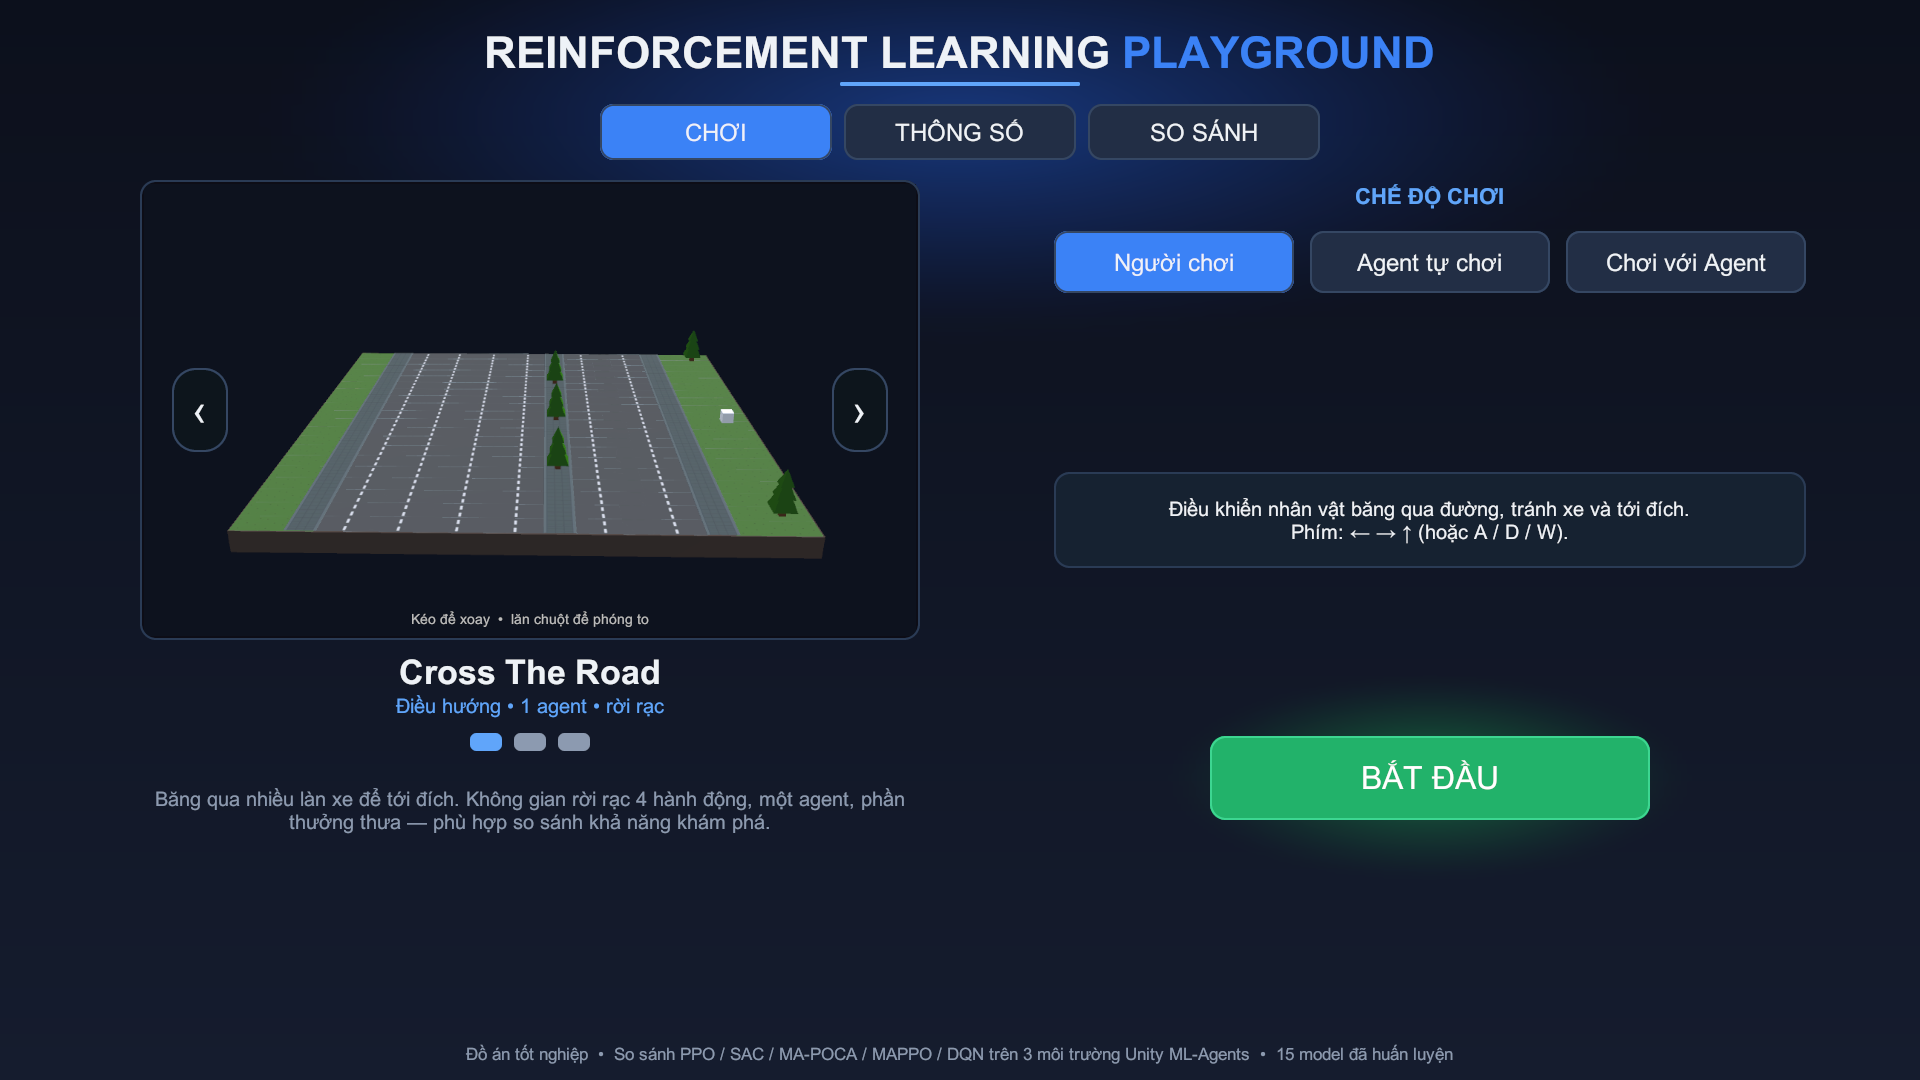
\includegraphics[width=0.85\textwidth]{image/app/app_menu_main.png}
\caption{Tab CHƠI của menu chính: khung xem trước ba chiều (trái) và các lựa
chọn chế độ chơi (phải)}
\label{fig:app_menu}
\end{figure}

{\sloppy
\indent Khung xem trước ba chiều là việc của thành phần Preview3D. Nó không dùng
ảnh tĩnh, mà nạp prefab môi trường từ thư mục \texttt{Resources/\allowbreak EnvPrefabs}
rồi chỉ sao chép các cặp lưới và vật liệu (MeshFilter và MeshRenderer)
sang một ``sân khấu'' đặt xa khu vực menu. Giữ lại mỗi phần hình học nghĩa là bản xem
trước không mang theo mã điều khiển hay thành phần vật lý nào; chẳng có mô phỏng nào chạy
ngầm, cũng không ảnh hưởng chéo tới scene menu. Một camera riêng render sân khấu ấy ra
RenderTexture rồi gắn vào giao diện, cho phép kéo chuột để xoay, lăn chuột để
phóng to; không thao tác gì thì mô hình tự xoay chậm. Khoảng cách camera ban đầu tính từ
hộp bao của toàn bộ hình khối, nên môi trường nào cũng vừa khung mà khỏi chỉnh tay. Hai
nút mũi tên hai bên khung cho phép nhảy nhanh giữa ba môi trường theo kiểu băng
chuyền.\par}

\indent Khu vực chọn mô hình chỉ hiện ra khi chế độ đang chọn có tác nhân máy tham gia. Số
ô chọn cũng đổi theo ngữ cảnh: tổ hợp nào chỉ cần một mô hình thì hiện một ô duy nhất,
riêng Football Table ở chế độ Agent tự chơi hiện hai ô riêng cho đội Xanh và đội
Đỏ (Hình~\ref{fig:app_menu_models}) để hai mô hình khác nhau đối đầu trực tiếp. Nhãn từng
ô cũng sinh theo ngữ cảnh: ``Model cho cả 2 agent'', ``Model đội Xanh'', ``Model agent đồng
đội''\dots{}, nên người dùng biết chính xác mô hình mình chọn sẽ điều khiển ai. Danh
sách mô hình trong mỗi ô liệt kê tự động từ thư mục tài nguyên, thành ra thêm một mô hình
mới chỉ là chuyện sao chép tệp ONNX vào đúng chỗ, không phải sửa dòng mã nào. Mỗi ô hiển
thị tên thuật toán ghép mã lần chạy, chẳng hạn ``MA-POCA \textperiodcentered{}
ctf\_poca\_v2'', và tô đúng màu quy ước của thuật toán đó. Duyệt lần lượt năm mô hình của
một môi trường, người dùng biết ngay đang xem chính sách của thuật toán nào, khỏi phải
thuộc lòng quy ước đặt tên các lần chạy.

\begin{figure}[H]
\centering
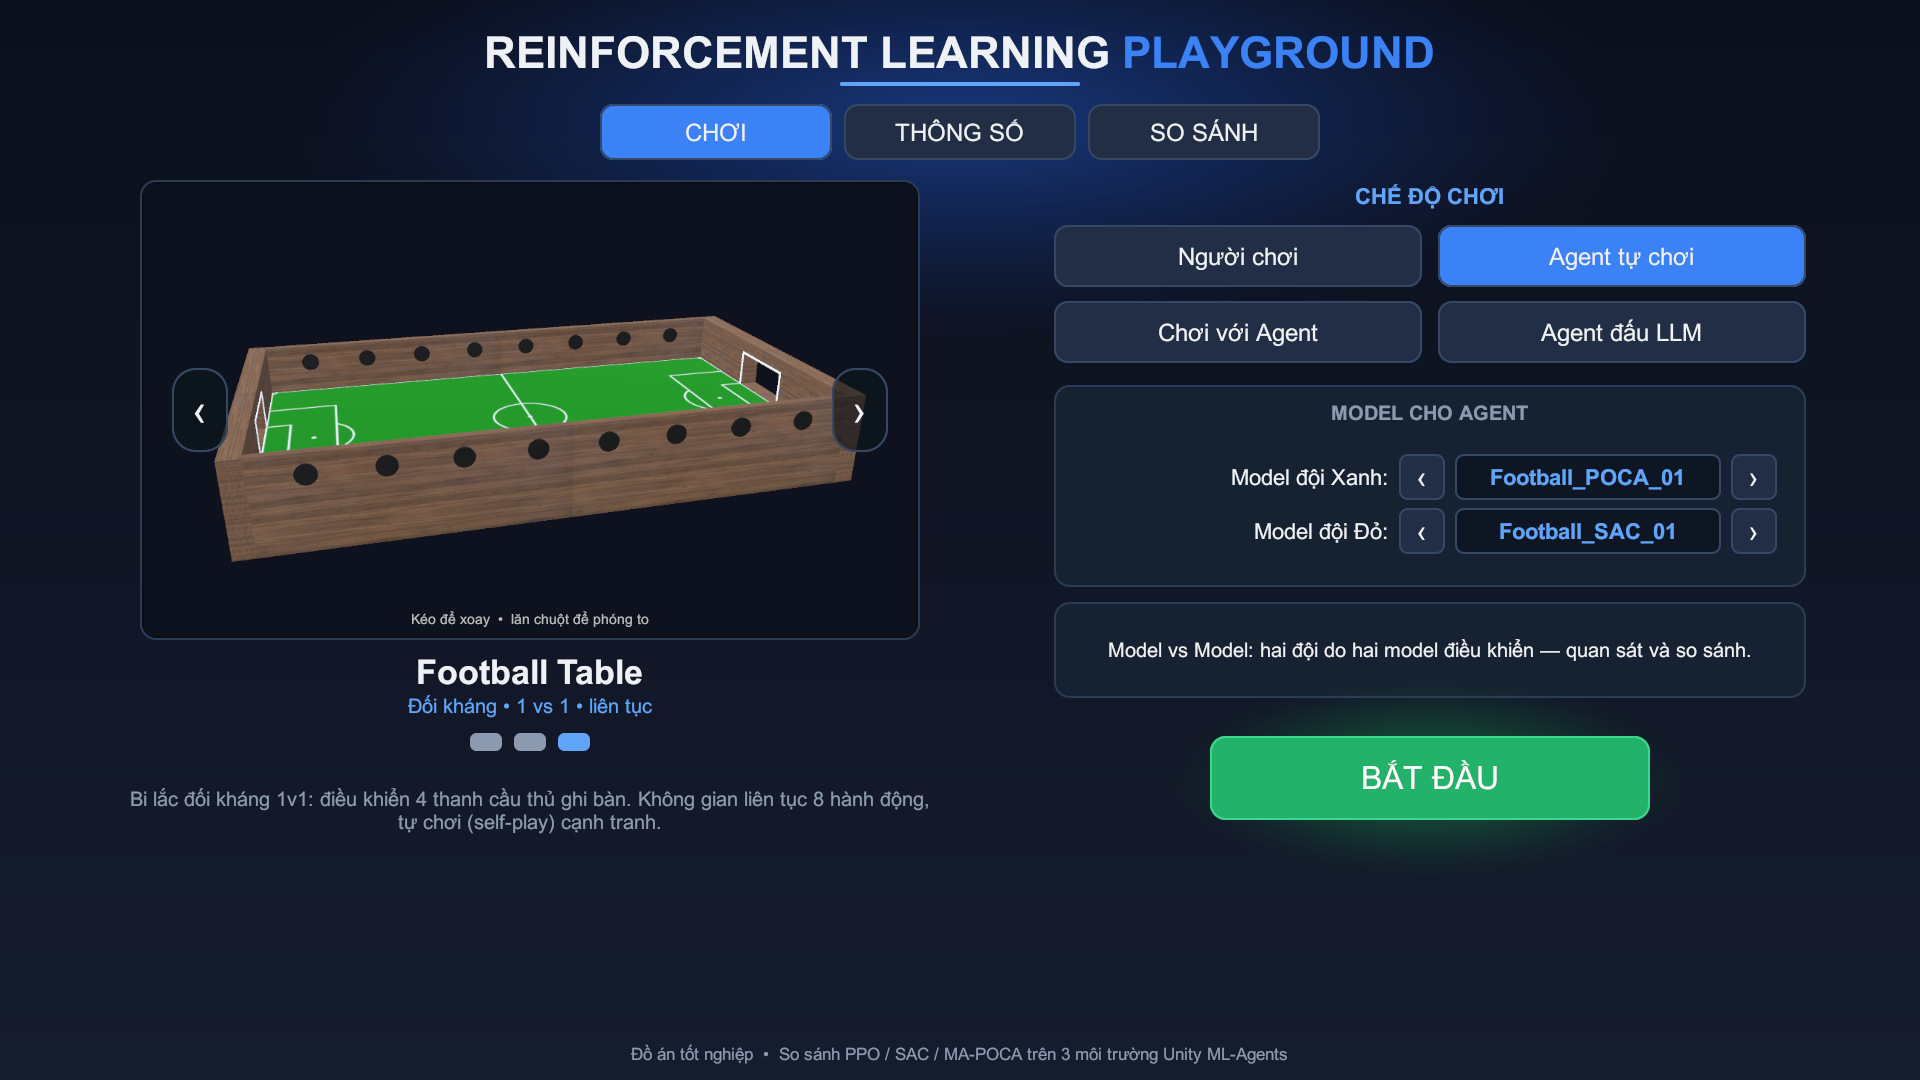
\includegraphics[width=0.85\textwidth]{image/app/app_menu_models.png}
\caption{Khu vực chọn mô hình khi Football Table ở chế độ Agent tự chơi:
hai ô chọn riêng cho đội Xanh và đội Đỏ}
\label{fig:app_menu_models}
\end{figure}

\indent Nút bắt đầu chỉ sáng lên khi mọi điều kiện đã đủ. Thư mục mô hình của môi trường
đang chọn mà rỗng, hoặc hai ô mô hình của Football Table rơi vào hai loại không gian hành
động khác nhau, thì ứng dụng khóa nút bắt đầu và hiện một dòng cảnh báo đỏ chỉ rõ nguyên
nhân. Nhờ vậy người dùng không rơi vào cảnh bấm chơi rồi mới gặp lỗi giữa chừng.

\indent Mọi phiên chơi đều có một thanh thông tin mỏng phủ ở mép trên màn hình: tên môi
trường, chế độ chơi, mô hình đang dùng, và nút quay về menu (hoặc phím Esc). Mép dưới là
dòng nhắc phím điều khiển. Người dùng vì thế luôn biết mình đang ở tổ hợp thực nghiệm nào,
và quay lại menu đổi lựa chọn lúc nào cũng được mà không phải khởi động lại ứng dụng.

% ───────────────────────────────────────────────
\subsection{Nạp mô hình ONNX tại thời gian chạy}
\label{sub:app-model}

\indent Mỗi lần huấn luyện ở Chương~\ref{ch:results} kết thúc, ML-Agents xuất chính sách
đã học ra một tệp ONNX. Muốn dùng được chúng trong ứng dụng thì phải sao chép vào cây thư
mục tài nguyên của Unity, theo quy ước mỗi môi trường một thư mục con:

\begin{center}
\texttt{Assets/GameHub/Resources/AgentModels/\{CrossTheRoad | CaptureTheFlag |
Football\}/}
\end{center}

{\sloppy
\noindent Tên tệp giữ đúng bằng mã của lần chạy huấn luyện, \texttt{ctr01} hay
\texttt{ctf\_mappo\_v2} chẳng hạn, và cũng chính tên đó là nhãn hiển thị trong menu. Mô
hình trong ứng dụng vì vậy luôn truy vết ngược được về đúng thư mục kết quả và đúng biểu
đồ đã phân tích ở Chương~\ref{ch:results}. Unity nhập mỗi tệp ONNX thành một tài sản
ModelAsset của gói suy luận tích hợp; ứng dụng nhờ đó liệt kê được danh sách mô
hình bằng cách gọi Resources.LoadAll, rồi gán mô hình đã chọn cho tác nhân qua
giao diện SetModel của ML-Agents, như đoạn mã dưới đây.\par}

\begin{lstlisting}[language={[Sharp]C}, caption={Liệt kê và gán mô hình ONNX tại thời gian chạy}]
ModelAsset[] models =
    Resources.LoadAll<ModelAsset>("AgentModels/" + envName);

agent.SetModel(behaviorName, selectedModel);
behaviorParameters.BehaviorType = BehaviorType.InferenceOnly;
\end{lstlisting}

\indent Cách tổ chức này tách hẳn dữ liệu mô hình khỏi mã nguồn. Danh mục mô hình trong
menu phản ánh trực tiếp nội dung thư mục tài nguyên, nên thêm mô hình mới chỉ là chuyện
sao chép tệp. Mà thao tác sao chép ấy giờ do chính kịch bản xuất dữ liệu huấn luyện lo
(Mục~\ref{sub:app-stats}): sau mỗi đợt huấn luyện, kịch bản lấy tệp ONNX cuối cùng của
từng lần chạy, đặt tên theo mã lần chạy, ghi vào đúng thư mục con của môi trường. Ứng dụng
nhờ đó luôn đóng gói toàn bộ $15$ mô hình ứng với $15$ lần chạy của
Chương~\ref{ch:results}, liệt kê ở Bảng~\ref{tab:app_models}. Mỗi môi trường có đủ năm
chính sách của năm thuật toán đặt cạnh nhau, so sánh hành vi bằng mắt ngay trên cùng một
nhiệm vụ.

\begin{table}[H]
\centering
\caption{$15$ mô hình ONNX được đóng gói sẵn trong ứng dụng}
\label{tab:app_models}
\renewcommand{\arraystretch}{1.3}
\tablefont
\begin{tabular}{|p{3.0cm}|p{4.6cm}|p{3.8cm}|>{\centering\arraybackslash}p{1.6cm}|}
\hline
\textbf{Môi trường} & \textbf{Tệp mô hình} & \textbf{Thuật toán} & \textbf{Số bước} \\
\hline
\multirow{5}{*}{Cross The Road}
 & \texttt{ctr01} & PPO & 2,00M \\
\cline{2-4}
 & \texttt{CrossTheRoad\_SAC\_01} & SAC & 2,00M \\
\cline{2-4}
 & \texttt{ctr\_poca\_v1} & MA-POCA & 2,00M \\
\cline{2-4}
 & \texttt{ctr\_mappo\_v1} & MAPPO & 2,00M \\
\cline{2-4}
 & \texttt{ctr\_dqn\_v1} & DQN & 2,00M \\
\hline
\multirow{5}{*}{Capture The Flag}
 & \texttt{ctf\_ppo\_v1} & PPO & 1,70M \\
\cline{2-4}
 & \texttt{ctf\_sac\_v1} & SAC & 1,64M \\
\cline{2-4}
 & \texttt{ctf\_poca\_v2} & MA-POCA & 1,70M \\
\cline{2-4}
 & \texttt{ctf\_mappo\_v2} & MAPPO & 1,70M \\
\cline{2-4}
 & \texttt{ctf\_dqn\_v1} & DQN & 1,70M \\
\hline
\multirow{5}{*}{Football Table}
 & \texttt{FB01} & PPO (self-play) & 1,60M \\
\cline{2-4}
 & \texttt{Football\_SAC\_01} & SAC (self-play) & 1,60M \\
\cline{2-4}
 & \texttt{Football\_POCA\_01} & MA-POCA (self-play) & 1,60M \\
\cline{2-4}
 & \texttt{Football\_MAPPO\_01} & MAPPO (self-play) & 1,60M \\
\cline{2-4}
 & \texttt{football\_dqn\_v1} & DQN (rời rạc) & 1,60M \\
\hline
\end{tabular}
\end{table}

\indent Một chi tiết kỹ thuật phải xử lý riêng khi đóng gói đủ $15$ mô hình là
không gian hành động. Trên Cross The Road và Capture The Flag, cả năm thuật
toán đều dùng hành động rời rạc nên mọi tệp ONNX đều nạp được vào scene gốc. Riêng
Football Table, bốn thuật toán PPO, SAC, MA-POCA và MAPPO sinh chính sách hành động
liên tục tám kênh, còn DQN chỉ định nghĩa được trên hành động rời rạc nên lần chạy
\texttt{football\_dqn\_v1} dùng phiên bản tám nhánh ba mức của cùng bài toán
(Mục~\ref{sub:env-football}). Không gian hành động được khai báo trong thành phần
BehaviorParameters của scene và ML-Agents dựng bộ truyền động của tác nhân
ngay trong pha OnEnable, tức trước khi ứng dụng kịp can thiệp sau khi scene
nạp xong; vì thế không thể đổi kiểu hành động tại thời gian chạy như cách đổi mô hình.
Giải pháp là giữ song song hai bản scene Football: bản liên tục dùng cho bốn thuật toán
kia và bản rời rạc FootballDiscrete sinh tự động từ bản gốc bằng một kịch bản
trong trình soạn thảo. Khi người dùng chọn mô hình DQN, menu nạp bản rời rạc thay cho
bản gốc; phần còn lại của ứng dụng không thay đổi vì lớp tác nhân của Football Table vốn đã
chấp nhận cả hai kiểu hành động và tự quy đổi ba mức $\{0,1,2\}$ về $\{-1,0,+1\}$. Hệ
quả duy nhất người dùng nhìn thấy là ở chế độ Agent tự chơi của Football Table,
hai ô chọn mô hình phải cùng loại hành động: menu khóa nút bắt đầu kèm dòng cảnh báo
nếu ghép DQN với một thuật toán liên tục, vì một trận đấu chỉ nạp được một scene.

% ───────────────────────────────────────────────
\subsection{Trực quan hóa kết quả huấn luyện trong ứng dụng}
\label{sub:app-stats}

\indent Thứ tách ứng dụng này khỏi một demo game thông thường là hai tab số liệu nhúng
thẳng vào menu. Số liệu hiển thị ở đó không do ai gõ tay, mà trích tự động từ chính các
tệp nhật ký huấn luyện. Mỗi lần huấn luyện lại, chỉ cần một lệnh là ứng dụng có số liệu
mới.

\subsubsection{Đường ống dữ liệu từ TensorBoard vào game}

\indent Khi huấn luyện, ML-Agents ghi các chỉ số ra tệp \texttt{tfevents} trong thư mục
\texttt{results/<run\_id>/}. Kịch bản Python \texttt{export\_training\_data.py} đọc những
tệp này bằng EventAccumulator của TensorBoard rồi chạy bốn bước xử lý nối tiếp.
Bước một, gộp chuỗi \texttt{Environment/Cumulative Reward} của mọi tệp nhật ký thuộc cùng
một lần chạy và sắp theo số bước. Bước hai, làm mượt chuỗi bằng trung bình trượt để bớt
nhiễu giữa các tập. Bước ba, rút gọn chuỗi đã làm mượt xuống tối đa $120$ điểm cách đều, giữ
kích thước tệp đủ nhỏ để nạp trong game. Bước bốn, tính các thống kê tóm tắt: phần thưởng
cuối, phần thưởng tốt nhất, trung bình mười phần trăm cuối, bước hội tụ ước
lượng, tổng số bước.

\indent Cũng trong lượt chạy đó, kịch bản làm thêm hai việc để dữ liệu và mô hình không
bao giờ lệch pha. Việc thứ nhất: sao chép tệp ONNX cuối cùng của từng lần chạy vào thư mục
tài nguyên của ứng dụng dưới đúng tên mã lần chạy, bỏ qua tệp đã trùng kích thước để Unity
khỏi nhập lại. Việc thứ hai: xác định không gian hành động của từng mô hình bằng cách đọc
thẳng tên tenxơ đầu ra trong tệp ONNX, rồi ghi kết quả vào JSON để ứng dụng biết trước mô
hình nào cần bản scene rời rạc. Có hai bước đó, một lệnh duy nhất sau mỗi đợt huấn luyện
là đủ để biểu đồ, bảng thống kê và danh mục mô hình trong menu cùng được cập nhật.

{\sloppy
\indent Kết quả cuối cùng gom vào đúng một tệp,
\texttt{Resources/\allowbreak TrainingData/\allowbreak training\_data.json}. Cấu trúc của
nó phân cấp: danh sách môi trường, mỗi môi trường một danh sách thuật toán, mỗi thuật toán
gồm mã lần chạy, tên tệp mô hình, không gian hành động, các thống kê tóm tắt, cùng hai
mảng song song \texttt{cs} (số bước) và \texttt{cv} (giá trị phần thưởng đã làm mượt). Tệp
hiện hành chứa đủ $15$ lần chạy của Chương~\ref{ch:results}. Bên phía Unity, lớp
TrainingDataStore nạp tệp một lần duy nhất bằng JsonUtility rồi lưu đệm.
Năm thuật toán đều có màu cố định (PPO xanh dương, SAC xanh lá, MA-POCA cam, MAPPO tím, DQN
đỏ), dùng thống nhất cho biểu đồ, chú giải lẫn bảng, và trùng với bảng màu của các đồ
thị ở Chương~\ref{ch:results} để người xem đối chiếu giữa hai nơi mà khỏi phải đọc lại chú
giải. Mã lần chạy được lưu kèm, nên mọi con số hiển thị trong ứng dụng đều truy ngược được
về đúng thư mục kết quả đã dùng phân tích ở Chương~\ref{ch:results}. Mã đó cũng chính là
tên tệp mô hình trong tab \textit{CHƠI}: từ một dòng trong bảng thống kê, người dùng chọn
ngay được mô hình tương ứng để xem nó chơi thật.\par}

\subsubsection{Tab THÔNG SỐ}

\indent Tab \textit{THÔNG SỐ} (Hình~\ref{fig:app_stats}) hiện đường cong phần thưởng tích
lũy của mọi thuật toán đã huấn luyện trên môi trường đang chọn, kèm bảng thống kê phía
dưới. Biểu đồ do thành phần UILineChart vẽ. Đây là một MaskableGraphic
tự sinh lưới tam giác trong hàm OnPopulateMesh: mỗi đoạn của đường cong dựng
thành một hình chữ nhật độ dày cố định, kèm lưới nền và trục. Vẽ trực tiếp bằng mesh như
vậy khiến biểu đồ không lệ thuộc thư viện đồ thị ngoài nào mà vẫn co giãn đúng theo kích
thước màn hình. Miền giá trị hai trục thì tính lại mỗi lần đổi môi trường, từ chính dữ
liệu đang vẽ, có đệm thêm mười phần trăm để đường cong không chạm mép khung.

\begin{figure}[H]
\centering
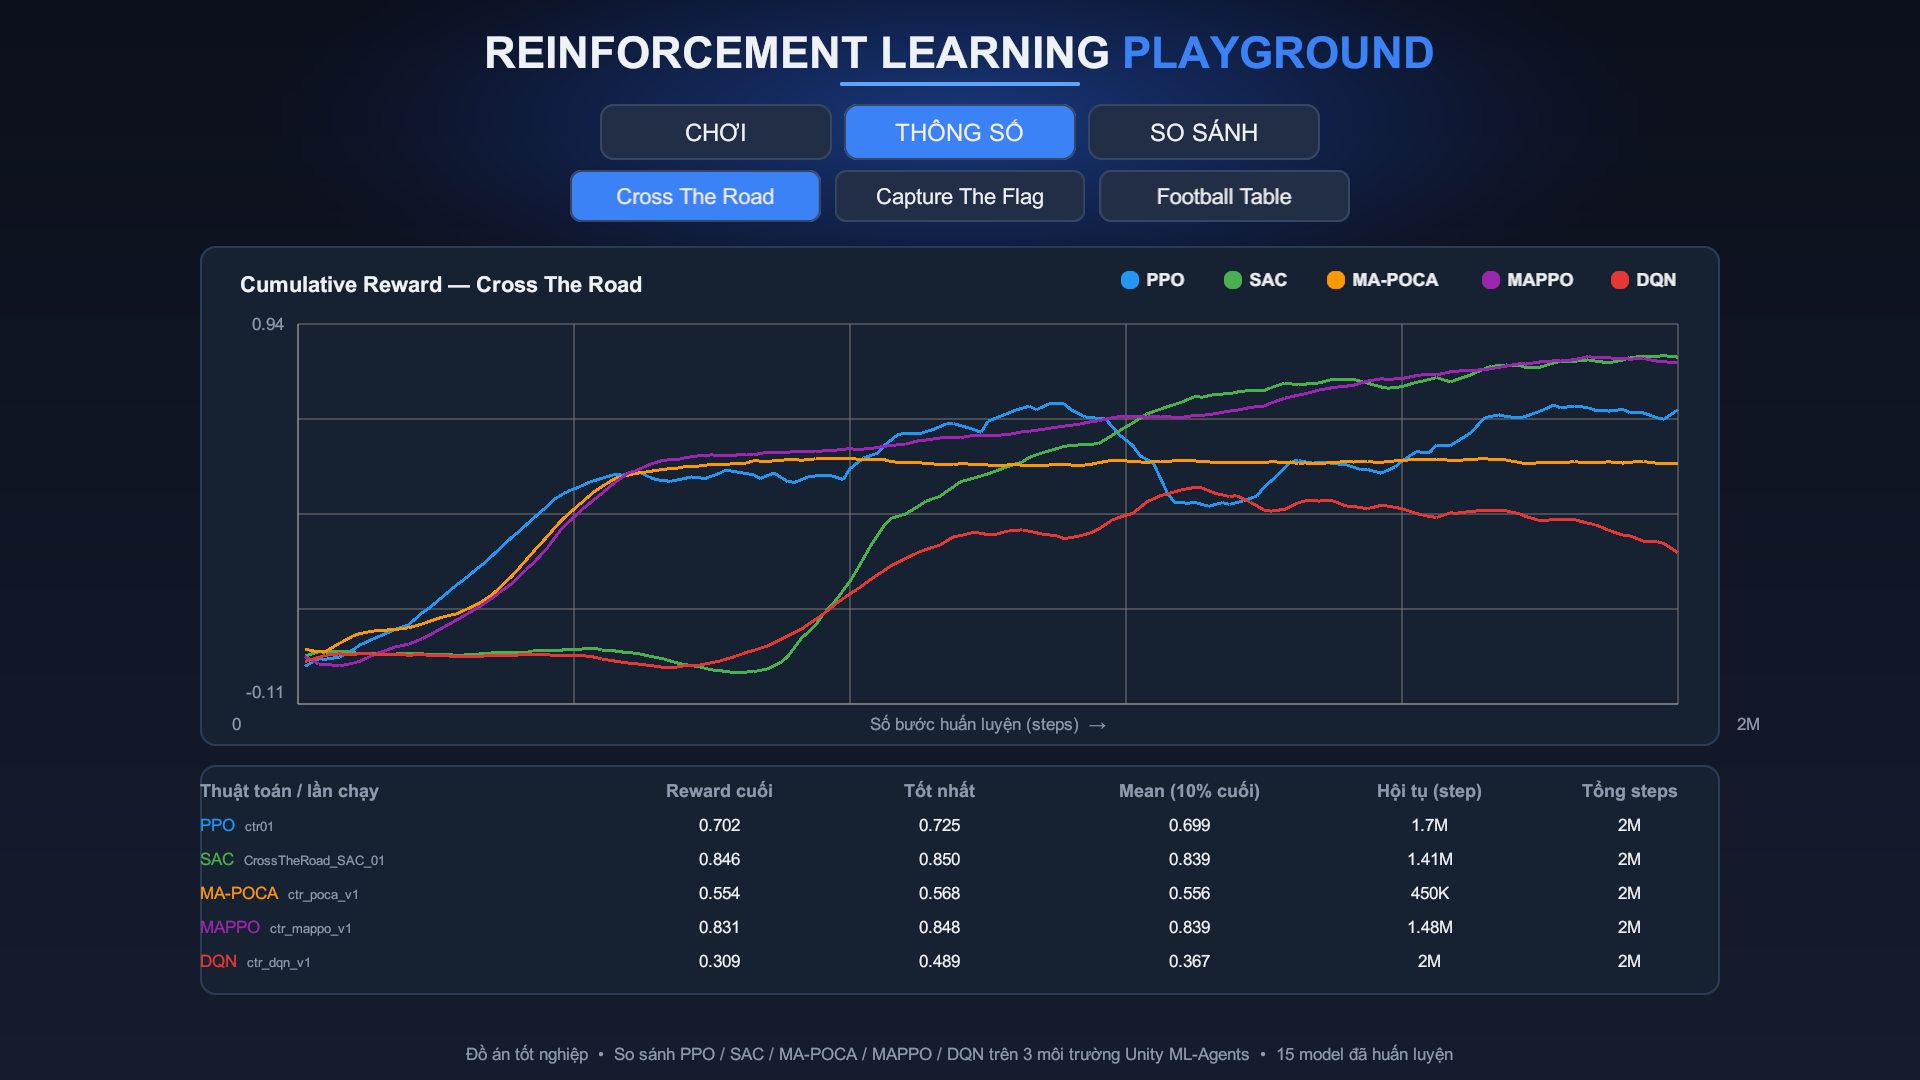
\includegraphics[width=0.97\textwidth]{image/app/app_menu_stats.png}
\caption{Tab THÔNG SỐ: đường cong phần thưởng tích lũy và bảng thống kê của
năm thuật toán trên môi trường Cross The Road}
\label{fig:app_stats}
\end{figure}

\indent Bảng thống kê nằm dưới biểu đồ, liệt kê theo từng thuật toán các cột: phần thưởng
cuối, phần thưởng tốt nhất, trung bình mười phần trăm cuối, bước hội tụ ước lượng, tổng số
bước. Cột đầu ghi tên thuật toán kèm mã lần chạy ở cỡ chữ nhỏ, để mỗi dòng chỉ đích danh
mô hình đã sinh ra con số đó. Thuật toán nào chưa huấn luyện trên môi trường đang xem thì
hiện ``N/A'' chứ không bị ẩn đi, để người xem thấy rõ phạm vi thực nghiệm của đề tài
tới đâu. Đại lượng vẽ ở đây là phần thưởng tích lũy môi trường
(\texttt{Environment/Cumulative Reward}) lấy nguyên từ nhật ký huấn luyện, nên thang giá
trị có thể lệch so với các đường cong phần thưởng ngoại sinh ở Chương~\ref{ch:results}.
Hai tab số liệu trong ứng dụng phục vụ tra cứu nhanh, không thay thế phần phân tích chi
tiết của báo cáo.

\subsubsection{Tab SO SÁNH}

\indent Tab \textit{SO SÁNH} (Hình~\ref{fig:app_compare}) đưa ba môi trường lên cùng
một màn hình. Mỗi môi trường là một thẻ chứa biểu đồ cột, mỗi cột là một thuật toán
với chiều cao tỉ lệ theo phần thưởng trung bình mười phần trăm cuối và được tô đúng
màu quy ước; giá trị số được ghi ngay trên đỉnh cột. Do thang phần thưởng của ba môi
trường rất khác nhau (Football Table dùng thang lớn hơn hẳn hai môi trường còn lại),
chiều cao cột được chuẩn hóa theo giá trị lớn nhất trong từng thẻ chứ không
dùng chung một trục; nhờ vậy việc so sánh luôn diễn ra trong nội bộ một môi trường,
đúng với nguyên tắc không so sánh chéo thang phần thưởng giữa các môi trường. Bảng phía
dưới chỉ sắp thứ tự mô tả theo phần thưởng của một seed, không được hiểu là kết luận thống
kê. Riêng DQN trên Football Table được gắn dấu sao, làm mờ cột và loại khỏi bảng thứ tự vì
mô hình dùng scene rời rạc, không huấn luyện bằng self-play. Bốn mô hình còn lại cũng không
được xếp hạng bằng ELO nội bộ, do mỗi lần chạy có một kho đối thủ khác nhau.

\begin{figure}[H]
\centering
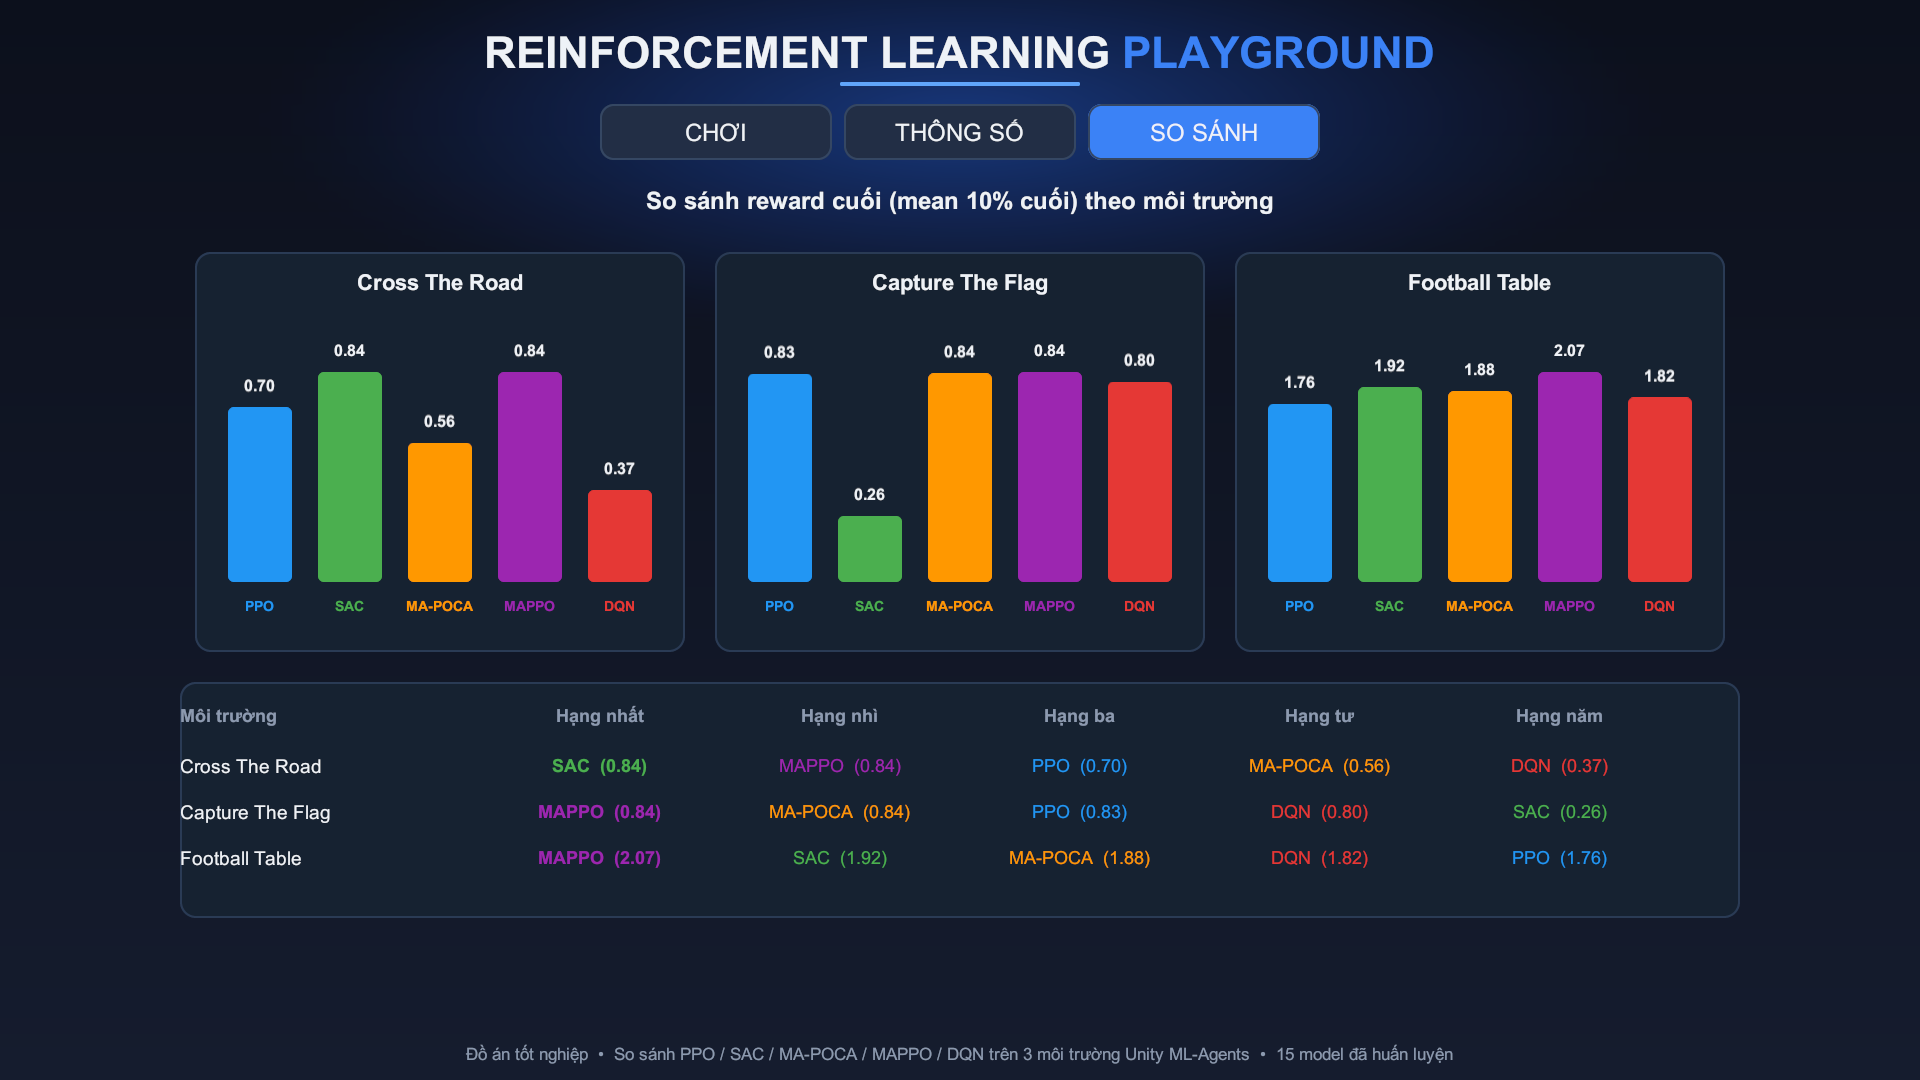
\includegraphics[width=0.97\textwidth]{image/app/app_menu_compare.png}
\caption{Tab SO SÁNH: các giá trị mô tả theo từng môi trường; DQN trên Football Table
được đánh dấu là tham chiếu riêng}
\label{fig:app_compare}
\end{figure}

% ───────────────────────────────────────────────
\subsection{Ba chế độ chơi trong từng môi trường}
\label{sub:app-modes}

\indent Ba môi trường khác nhau về bản chất (đơn tác nhân, hợp tác, đối kháng) nên ba chế độ
chơi phải ánh xạ vào mỗi nơi theo một cách riêng. Bảng~\ref{tab:app_mode_matrix}
tổng hợp lại.

\begin{table}[H]
\centering
\caption{Ánh xạ ba chế độ chơi vào ba môi trường}
\label{tab:app_mode_matrix}
\renewcommand{\arraystretch}{1.35}
\tablefont
\begin{tabular}{|>{\raggedright\arraybackslash}p{2.4cm}
                |>{\raggedright\arraybackslash}p{3.6cm}
                |>{\raggedright\arraybackslash}p{3.6cm}
                |>{\raggedright\arraybackslash}p{3.6cm}|}
\hline
\textbf{Môi trường} & \textbf{Người chơi} & \textbf{Agent tự chơi} & \textbf{Chơi với Agent} \\
\hline
Cross The Road & Người điều khiển nhân vật trong khu vực & Mô hình điều khiển nhân vật trong khu vực & Người và tác nhân đua song song ở hai khu vực liền kề \\
\hline
Capture The Flag & Hai người chơi trên cùng bàn phím & Hai tác nhân cùng dùng một mô hình & Người phối hợp cùng tác nhân đồng đội \\
\hline
Football Table & Người đấu với bot luật đơn giản & Mô hình đấu với mô hình (cùng loại hành động)$^{*}$ & Người đấu với mô hình \\
\hline
\multicolumn{4}{|p{14.2cm}|}{$^{*}$ Hai ô mô hình phải cùng dùng hành động liên tục
hoặc cùng rời rạc, vì mỗi loại chạy trên một bản scene riêng; xem
Mục~\ref{sub:app-model}.} \\
\hline
\end{tabular}
\end{table}

\subsubsection{Cross The Road: trải nghiệm và quan sát chính sách}

\indent Chế độ Người chơi cho người dùng điều khiển nhân vật bằng phím mũi tên
(hoặc A/D/W), đúng theo bốn hành động rời rạc mà tác nhân được phép dùng khi huấn luyện:
đứng yên, sang trái, sang phải, tiến lên. Ràng buộc người chơi vào đúng không gian hành
động của tác nhân là chủ ý, có thế người dùng mới đánh giá đúng độ khó của bài toán, chứ
được điều khiển tự do hơn tác nhân thì rất dễ đi tới kết luận sai lệch.

\indent Chế độ Agent tự chơi chuyển mọi tác nhân trong scene sang suy luận bằng
mô hình đã chọn, đồng thời camera tự đóng khung vào vùng chơi
(Hình~\ref{fig:app_ctr_agent}). Thanh thông tin phía trên hiện tên mô hình đang chạy; bảng
chỉ số dựng sẵn trong môi trường hiện phần thưởng tích lũy, số tập đã hoàn thành và số
bước của tập hiện tại. Người xem nhờ vậy đối chiếu được ngay hành vi quan sát được với chỉ
số mà mô hình đạt. Đây cũng là cách trực quan nhất để thấy khác biệt giữa các thuật toán:
mô hình SAC băng qua đường với ít va chạm hơn, còn mô hình MAPPO hay dừng lâu hơn ở những
làn mật độ phương tiện cao, khớp với thứ hạng phần thưởng đã trình bày ở
Chương~\ref{ch:results}.

\begin{figure}[H]
\centering
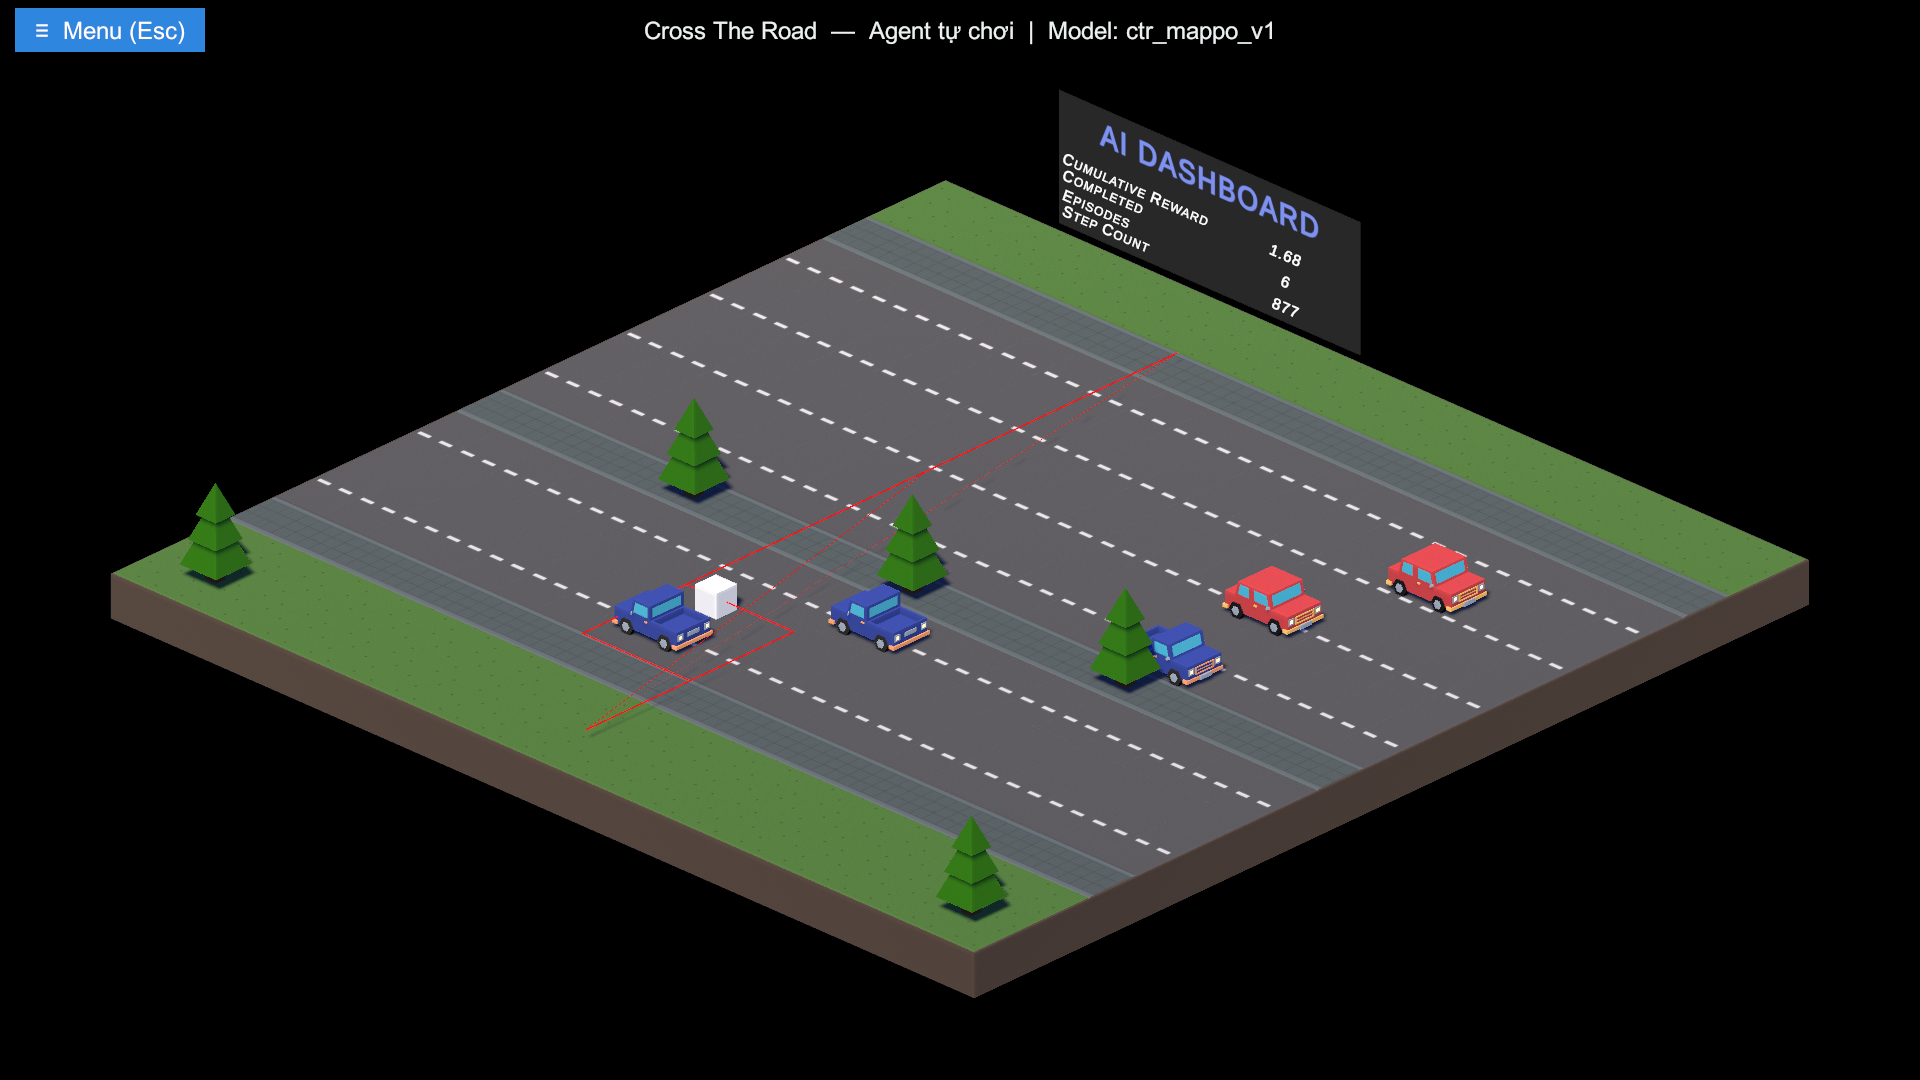
\includegraphics[width=0.78\textwidth]{image/app/app_ctr_agent.png}
\caption{Chế độ Agent tự chơi trong Cross The Road: mô hình
\texttt{ctr\_mappo\_v1} điều khiển tác nhân, chỉ số hiển thị trực tiếp trong cảnh}
\label{fig:app_ctr_agent}
\end{figure}

\indent Chế độ còn lại, Chơi với Agent, thiết kế theo kiểu đua song song. Ứng
dụng giữ lại hai khu vực huấn luyện cạnh nhau và tắt số còn lại, giao khu vực bên trái cho
người chơi, khu vực bên phải cho tác nhân máy, rồi tính lại khung nhìn sao cho cả hai cùng
nằm gọn trong màn hình. Scene Cross The Road hiện có tám khu vực huấn luyện nên chế độ này
dùng được thoải mái; số khu vực dư chẳng ảnh hưởng gì vì chúng bị tắt ngay khi scene nạp
xong.

\subsubsection{Capture The Flag: phối hợp người và máy}

\indent Môi trường hợp tác mở ra một kịch bản khá thú vị: con người phối hợp với tác nhân
máy trong cùng một đội. Ở chế độ Chơi với Agent, người chơi cầm một nhân vật bằng
phím W A S D (kèm Q/E để đi ngang), nhân vật thứ hai do mô hình đã chọn điều khiển
(Hình~\ref{fig:app_ctf_pva}). Nhiệm vụ đòi hỏi đúng chuỗi phối hợp đã phân tích ở
Mục~\ref{sub:env-coop}: một bên đứng lên bàn đạp giữ cửa, bên kia đi qua, rồi đổi vai.
Người chơi vì thế phải đoán được ý định của đồng đội máy và hành động sao cho ăn khớp,
minh họa trực tiếp cho khái niệm phối hợp đa tác nhân.

\begin{figure}[H]
\centering
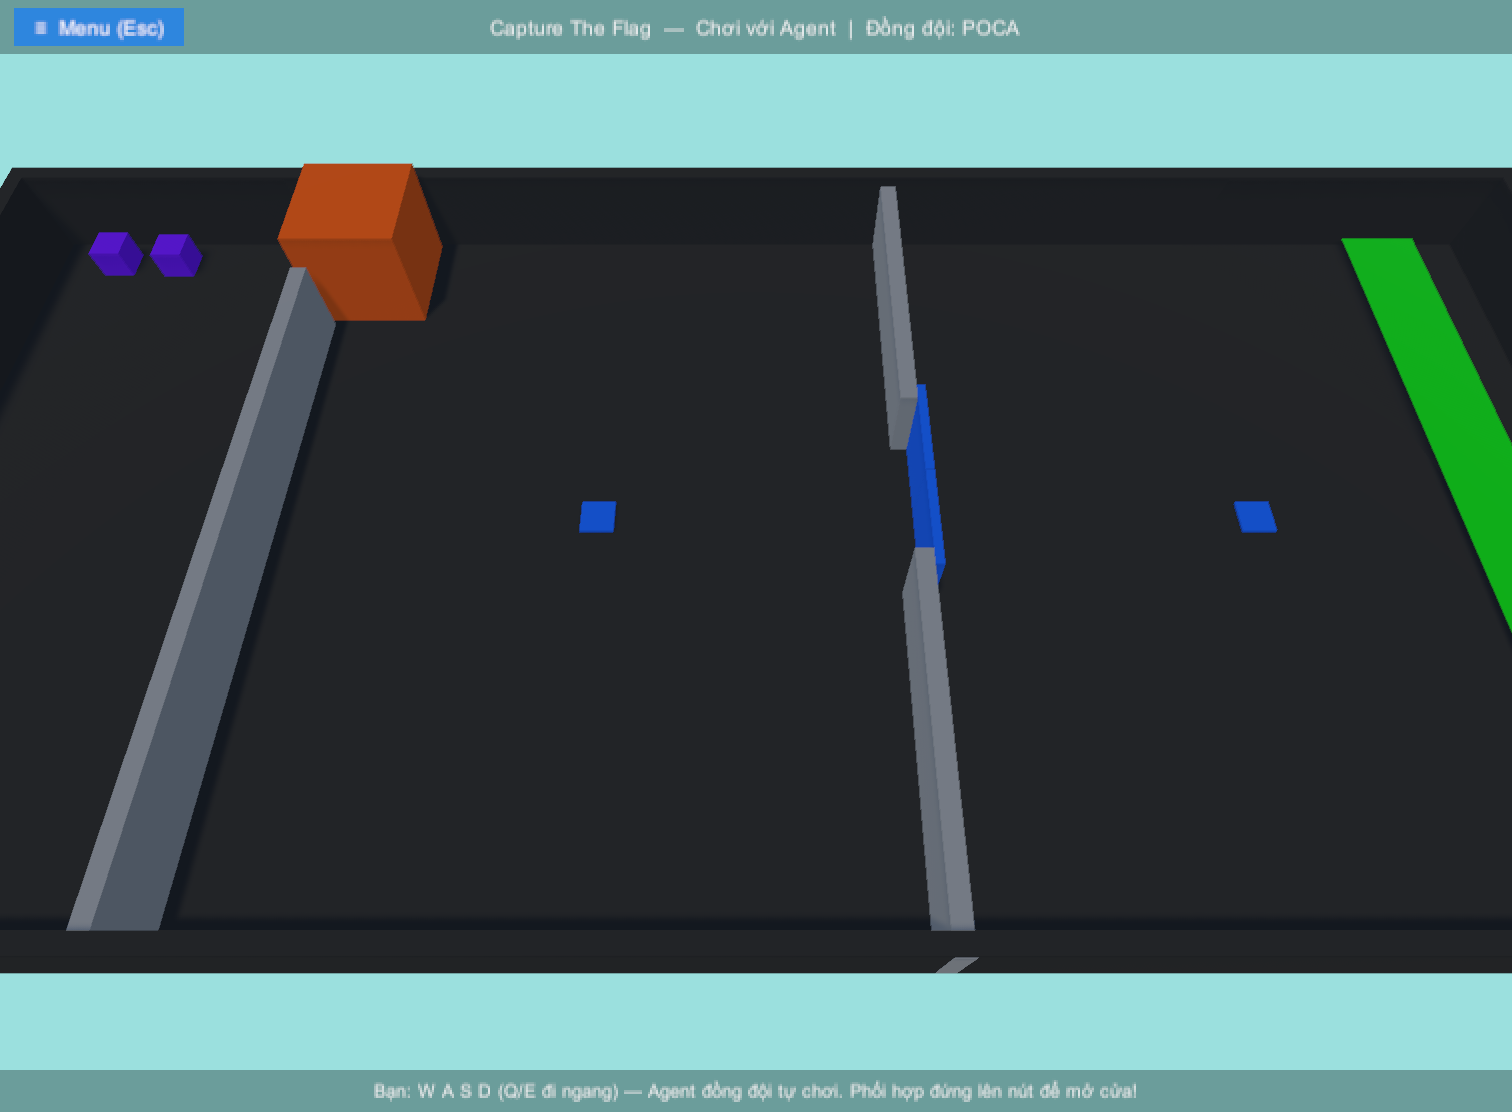
\includegraphics[width=0.78\textwidth]{image/app/app_ctf_pva.png}
\caption{Chế độ Chơi với Agent trong Capture The Flag: người chơi phối hợp
cùng tác nhân đồng đội dùng mô hình \texttt{ctf\_mappo\_v2}}
\label{fig:app_ctf_pva}
\end{figure}

\indent Chế độ Người chơi thì cả hai nhân vật đều do con người cầm, kiểu hai
người chơi chung một bàn phím: một người dùng cụm W A S D (Q/E đi ngang), người kia dùng
cụm phím mũi tên (dấu ngoặc vuông để đi ngang). Còn chế độ Agent tự chơi giao cả
hai nhân vật cho cùng một mô hình, tái hiện đúng cấu hình lúc huấn luyện, vì hai tác nhân
vốn dùng chung một chính sách.

\subsubsection{Football Table: đối đầu người với máy và máy với máy}

\indent Ở môi trường đối kháng, chế độ Chơi với Agent cho người chơi cầm đội Xanh
đấu trực tiếp với mô hình bên đội Đỏ. Mỗi đội có bốn thanh gạt với tám kênh điều khiển
liên tục, nên sơ đồ phím phải theo nguyên tắc ``một thanh tại một thời điểm'': phím Q/E
hoặc các phím số 1-4 chọn thanh đang điều khiển, W/S trượt thanh, A/D xoay thanh để sút
(Hình~\ref{fig:app_fb_player}). Tên thanh đang chọn (thủ môn, hậu vệ, tiền vệ, tiền đạo) hiện
ở góc trên trái màn hình. Giá trị hành động do người chơi sinh ra còn được nhân với
dấu của đội, y như cách chuẩn hóa hệ tọa độ khi huấn luyện, nên cùng một sơ đồ phím dùng
được cho cả hai phía sân. Sang chế độ Người chơi, đối thủ là bot luật cố định bám
theo vị trí bóng, đúng đối thủ mốc đã dùng khi huấn luyện ở Mục~\ref{sub:env-football}.
Độ khó vừa phải, hợp để người dùng làm quen sơ đồ điều khiển trước khi đối đầu các mô hình
đã huấn luyện.

\begin{figure}[H]
\centering
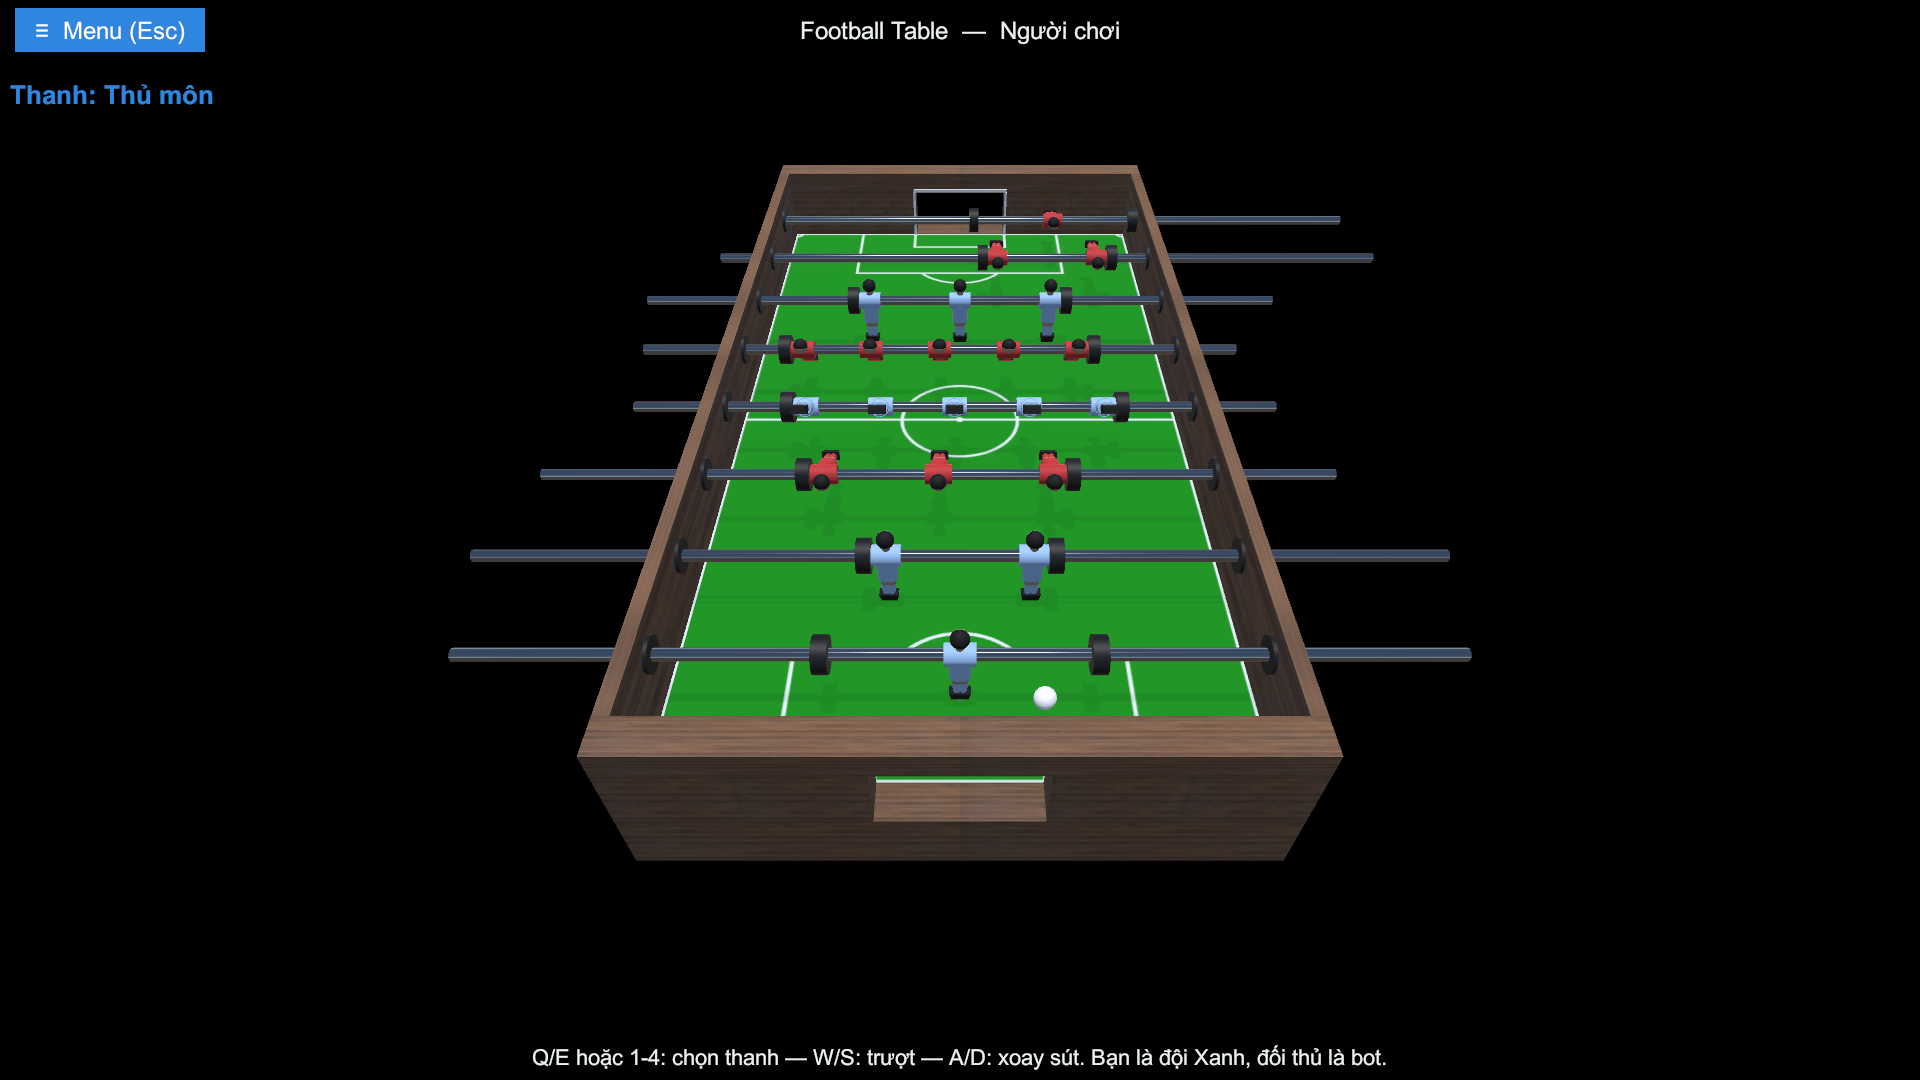
\includegraphics[width=0.78\textwidth]{image/app/app_fb_player.png}
\caption{Chế độ Người chơi trong Football Table: người chơi cầm đội Xanh,
góc trên trái hiển thị thanh gạt đang được chọn}
\label{fig:app_fb_player}
\end{figure}

\indent Thú vị nhất là chế độ Agent tự chơi với hai ô chọn mô hình độc lập. Người
dùng có thể cho mô hình PPO huấn luyện bằng tự chơi đấu với MA-POCA, MAPPO hay SAC, hoặc
cho hai bản sao của cùng một mô hình gặp nhau; thanh thông tin phía trên hiện tên mô hình
của cả hai đội cùng lúc. Riêng DQN chỉ đấu được với chính nó, vì đây là chính sách rời rạc
duy nhất trên môi trường này, và trận đấu ấy chạy trên bản scene rời rạc
(Hình~\ref{fig:app_fb_dqn}). Về bản chất, đây là một công cụ đánh giá đối kháng trực tiếp
thu nhỏ, bổ sung kênh so sánh định tính cho các kết quả định lượng ở Chương~\ref{ch:results},
bởi hai mô hình có phần thưởng trung bình sát nhau vẫn có thể
cho ra thế trận rất khác khi gặp trực tiếp.

\begin{figure}[H]
\centering
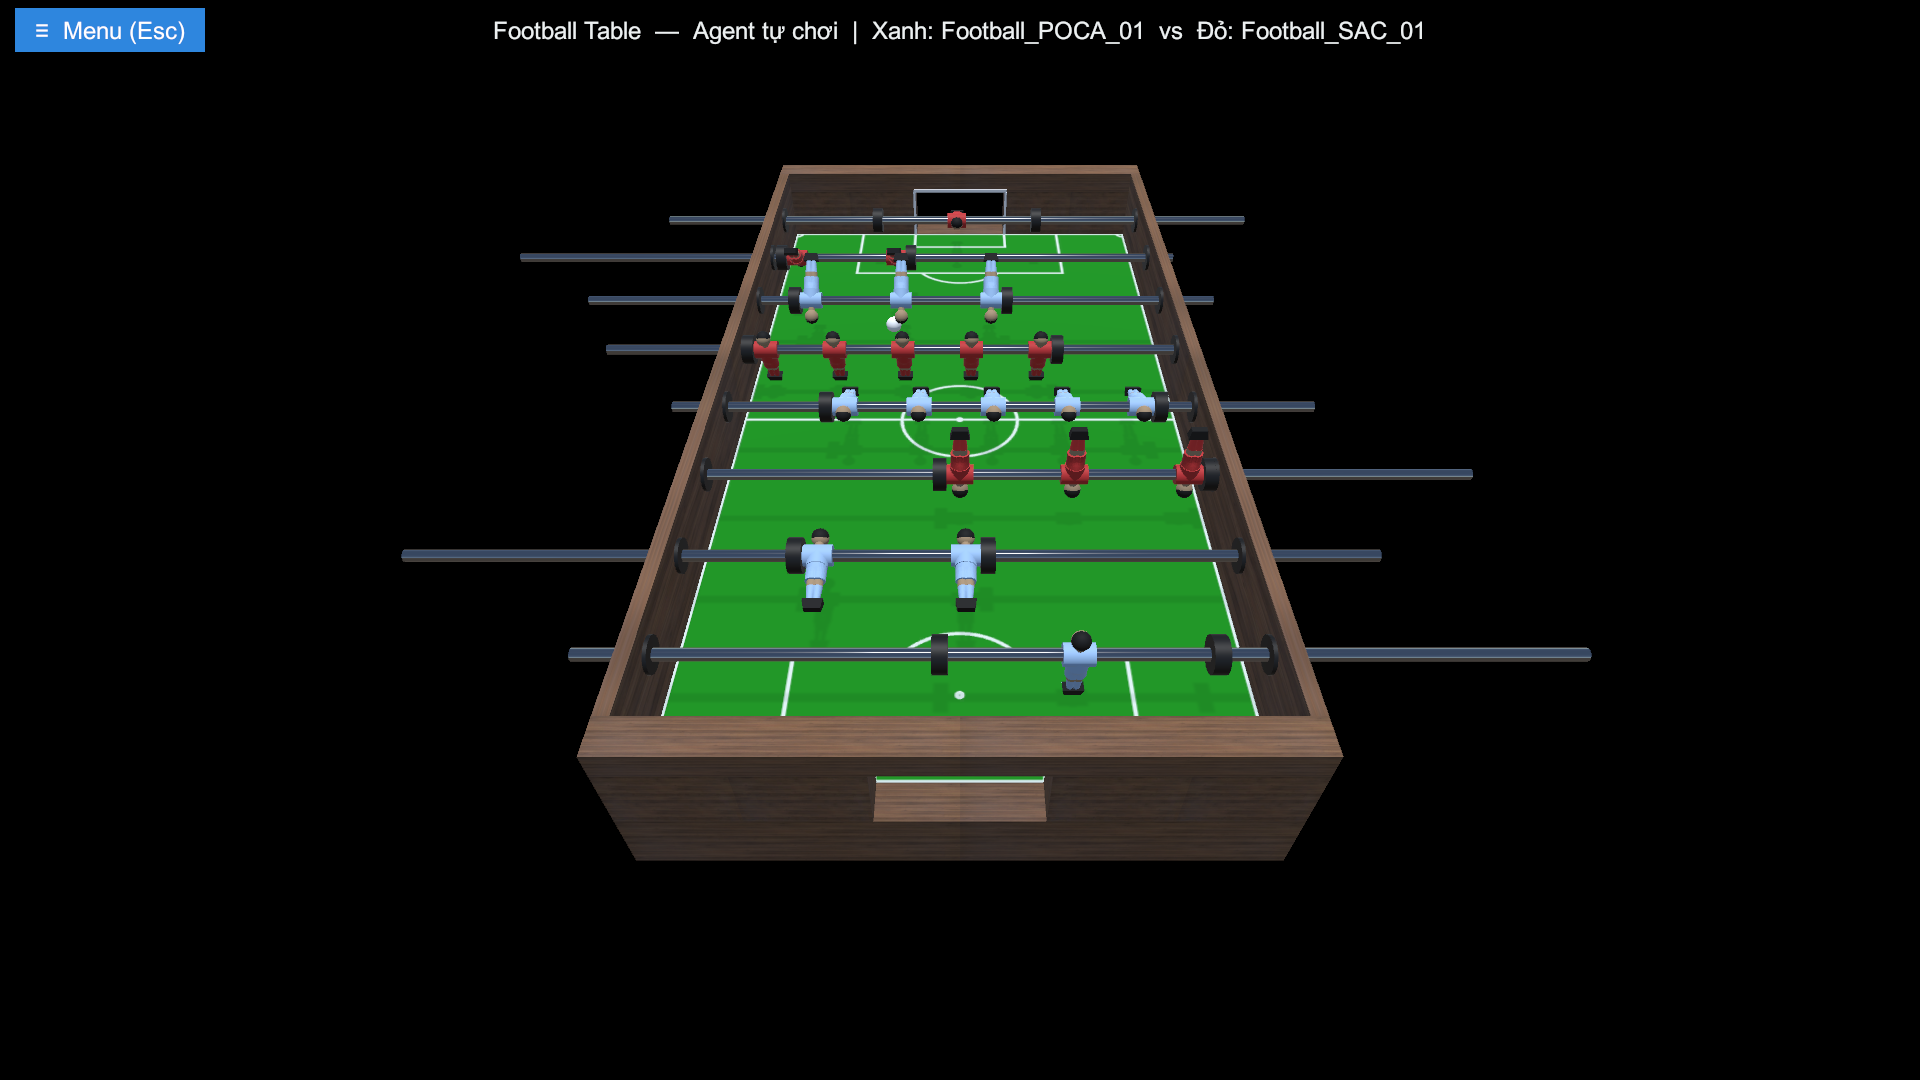
\includegraphics[width=0.78\textwidth]{image/app/app_fb_agent.png}
\caption{Chế độ Agent tự chơi trong Football Table với mô hình
\texttt{football\_dqn\_v1}: ứng dụng nạp bản scene rời rạc và chỉ giữ lại một bàn
trong số tám bàn của cấu hình huấn luyện}
\label{fig:app_fb_dqn}
\end{figure}

% ───────────────────────────────────────────────
\subsection{Đóng gói ba môi trường thành gói dùng lại được}
\label{sub:app-package}

\indent Ba môi trường của đề tài sinh ra cho một mục đích cụ thể là so sánh thuật toán,
nhưng bản thân chúng có giá trị dùng lại. Một lập trình viên Unity muốn thử học tăng cường
thường tiêu phần lớn thời gian ở khâu dựng môi trường, không phải ở khâu chọn thuật
toán. Vì thế đề tài gói cả ba môi trường thành một gói UPM (Unity Package
Manager) mang tên com.vanhuyen.rl-game-envs, cài được vào bất kỳ dự án Unity nào
như mọi gói chính thức khác.

\subsubsection{Cấu trúc gói}

\indent Gói theo đúng bố cục chuẩn của UPM, tóm tắt ở Bảng~\ref{tab:pkg_layout}. Nhưng
điểm đáng nói không phải danh sách thư mục, mà là ranh giới giữa chúng. Toàn bộ mã điều
khiển môi trường nằm trong Runtime và biên dịch thành một assembly riêng, tách
khỏi Assembly-CSharp của dự án. Nhờ vậy chính trình biên dịch canh giữ tính độc
lập của gói: một lớp môi trường lỡ tham chiếu tới mã của ứng dụng trình diễn là dự án hỏng
biên dịch ngay, chứ không phải đợi tới khi ai đó cài gói mới lòi ra.

\begin{table}[H]
\centering
\caption{Bố cục gói \texttt{com.vanhuyen.rl-game-envs}}
\label{tab:pkg_layout}
\renewcommand{\arraystretch}{1.3}
\tablefont
\begin{tabular}{|p{3.6cm}|>{\raggedright\arraybackslash}p{9.9cm}|}
\hline
\textbf{Thư mục} & \textbf{Nội dung} \\
\hline
\texttt{Runtime/} & 36 lớp điều khiển của ba môi trường (tác nhân, quan sát, hàm
phần thưởng, sinh vật cản, trọng tài) cùng giao diện
\texttt{IManualActionSource}; một assembly riêng. \\
\hline
\texttt{Editor/} & Trình hướng dẫn cài đặt và bốn công cụ: nhân khu vực huấn luyện,
build headless, sinh bản scene hành động rời rạc, cài cấu hình huấn luyện. \\
\hline
\texttt{Configs/} & $15$ tệp YAML cho năm thuật toán trên ba môi trường. \\
\hline
\texttt{Samples\textasciitilde/} & Bốn mẫu import được từ Package Manager: ba môi
trường (scene, prefab, vật liệu, thiết lập vật lý) và bộ cấu hình huấn luyện. \\
\hline
\texttt{Documentation\textasciitilde/} & Tài liệu hướng dẫn cài đặt, yêu cầu phiên bản
và phần cứng, thời gian huấn luyện tham khảo, checklist kiểm thử và giới hạn tái sử dụng;
kèm \texttt{README}, \texttt{CHANGELOG} và \texttt{LICENSE} ở gốc gói. \\
\hline
\end{tabular}
\end{table}

\subsubsection{Gỡ phụ thuộc ngược từ môi trường vào ứng dụng}

\indent Trước khi tiến hành đóng gói, đề tài cần xử lý một quan hệ phụ thuộc chưa phù hợp tồn tại trong kiến trúc ban đầu. Cụ thể, hàm Heuristic của cả ba tác nhân trực tiếp sử dụng GetComponent để truy cập các lớp cụ thể thuộc ứng dụng trình diễn nhằm thu nhận hành động điều khiển từ người dùng. Cách tổ chức này tạo ra quan hệ phụ thuộc ngược với phân tầng kiến trúc mong muốn: mã nguồn của môi trường thuộc tầng cơ sở và do đó không nên phụ thuộc vào ứng dụng sử dụng hoặc tích hợp môi trường. Trong phạm vi một dự án Unity đơn lẻ, sự phụ thuộc này có thể chưa gây ra vấn đề đáng kể; tuy nhiên, khi môi trường được tách thành một gói độc lập, nó dẫn đến lỗi biên dịch do assembly của gói không thể tham chiếu trực tiếp đến các lớp nằm trong assembly mặc định của dự án sử dụng.

\indent Để khắc phục vấn đề trên, đề tài áp dụng nguyên tắc đảo ngược phụ thuộc bằng cách định nghĩa một giao diện chung ngay trong gói:

\begin{lstlisting}[language={[Sharp]C}, caption={Giao diện cho nguồn điều khiển thủ công}]
public interface IManualActionSource
{
void WriteActions(in ActionBuffers actionsOut);
}
\end{lstlisting}

\indent Sau thay đổi này, hàm Heuristic của môi trường không còn phụ thuộc vào bất kỳ lớp điều khiển cụ thể nào của ứng dụng. Thay vào đó, tác nhân kiểm tra xem trên GameObject hiện tại có thành phần nào triển khai giao diện IManualActionSource hay không. Nếu tồn tại, thành phần đó được sử dụng để cung cấp hành động; trong trường hợp ngược lại, môi trường sử dụng sơ đồ điều khiển bàn phím mặc định. Theo cách tiếp cận này, ứng dụng trình diễn chỉ đóng vai trò là một bên triển khai giao diện, tương tự như các nguồn điều khiển khác, thay vì trở thành một phụ thuộc trực tiếp của môi trường.

\indent Thiết kế trên đồng thời tạo ra một điểm mở rộng thống nhất cho người sử dụng gói. Khi cần bổ sung một cơ chế điều khiển mới, chẳng hạn gamepad, kịch bản kiểm thử tự động hoặc một mô hình ngôn ngữ lớn, người dùng chỉ cần xây dựng một MonoBehaviour triển khai IManualActionSource và gắn thành phần đó vào đối tượng tương ứng. Nhờ đó, các phương thức điều khiển mới có thể được tích hợp mà không yêu cầu sửa đổi mã nguồn cốt lõi của môi trường, qua đó giảm mức độ liên kết giữa các thành phần và cải thiện khả năng mở rộng của gói.

\indent Bên cạnh việc đảo ngược phụ thuộc, quá trình đóng gói còn cần xử lý sự khác biệt giữa hai không gian hành động của môi trường Football Table đã trình bày tại Mục~\ref{sub:app-model}. Nếu mỗi nguồn điều khiển phải tự xác định và ghi hành động theo không gian liên tục hoặc rời rạc, logic chuyển đổi giữa các biểu diễn hành động sẽ bị lặp lại tại nhiều vị trí. Để tránh sự trùng lặp này, gói cung cấp một hàm tiện ích thực hiện quá trình chuyển đổi tập trung. Theo đó, nguồn điều khiển chỉ cần biểu diễn ý định điều khiển dưới dạng giá trị liên tục trong khoảng $[-1,1]$; việc ánh xạ các giá trị này sang không gian hành động phù hợp với brain đang được sử dụng sẽ do gói đảm nhiệm. Cách tổ chức này giúp thống nhất giao diện điều khiển, giảm mã nguồn lặp lại và tách biệt nguồn sinh hành động khỏi cách biểu diễn hành động cụ thể của tác nhân.


\subsubsection{Hướng dẫn cài đặt và sử dụng gói}
\label{subsub:pkg-usage}

\indent Rào cản lớn nhất với người mới không phải thiếu tài liệu, mà là không biết mình
đang đứng ở đâu trong tài liệu đó. Đề tài vì thế viết một cửa sổ Editor
(Hình~\ref{fig:pkg_wizard}) chia toàn bộ quy trình thành bảy bước. Mấu chốt nằm ở chỗ mỗi
bước tự kiểm tra trạng thái hiện tại rồi hiện dấu tích hoặc nút hành động tương
ứng chứ không chỉ liệt kê việc cần làm.

\begin{figure}[H]
\centering
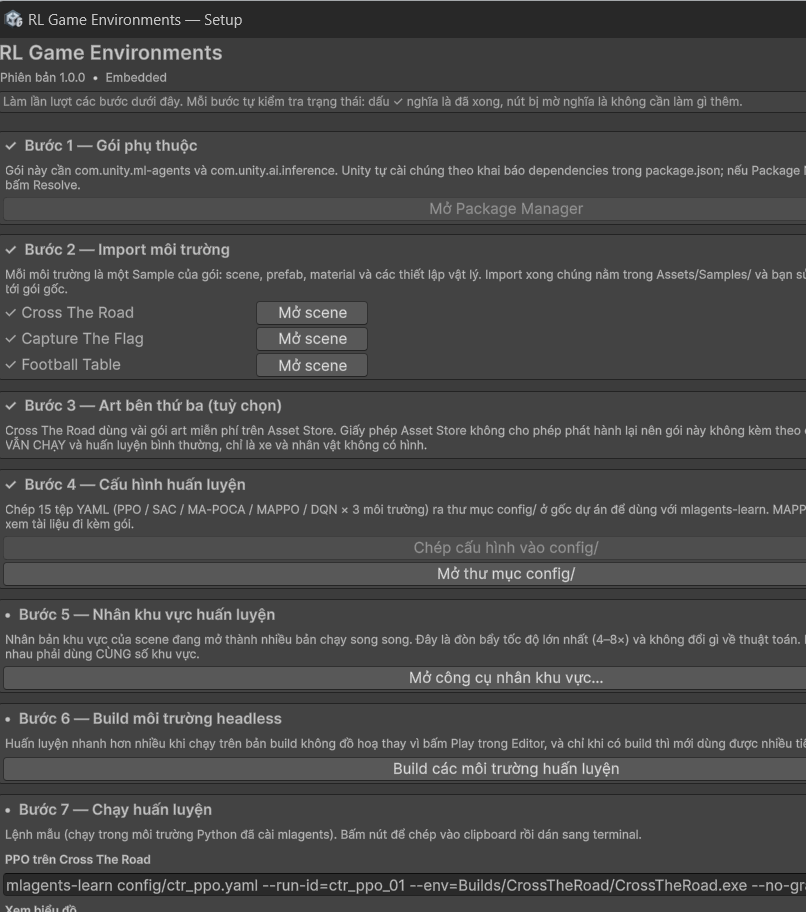
\includegraphics[width=0.82\textwidth]{image/app/app_pkg_wizard.png}
\caption{Trình hướng dẫn cài đặt của gói: bảy bước, mỗi bước tự kiểm tra trạng thái
và chỉ bật nút khi thực sự còn thiếu}
\label{fig:pkg_wizard}
\end{figure}

\indent Bảy bước lần lượt gồm: kiểm tra gói phụ thuộc; import môi trường từ mục Samples
của Package Manager; kiểm tra các gói art bên thứ ba; chép cấu hình huấn luyện ra thư mục
config; nhân khu vực huấn luyện; build môi trường headless; và cuối cùng là lệnh
mẫu để chạy huấn luyện, kèm nút chép sang clipboard. Ba bước giữa gọi lại đúng những công
cụ mà đề tài đã dùng cho phần thực nghiệm của chính mình, nghĩa là người dùng gói đi theo
một quy trình đã được kiểm chứng, chứ không phải quy trình viết riêng cho tài liệu.

\indent Quy trình sử dụng đầy đủ của gói được thực hiện như sau:

\begin{enumerate}
    \item Trong Unity Package Manager, chọn Add package from disk và trỏ tới
    tệp package.json của com.vanhuyen.rl-game-envs; nếu gói được đặt
    trong một kho Git có thể dùng Add package from git URL.
    \item Mở \texttt{Tools > RL Game Environments > Setup Wizard}, xác nhận hai phụ
    thuộc com.unity.ml-agents và com.unity.ai.inference, sau đó import
    môi trường cần dùng từ mục Samples của Package Manager.
    \item Chép bộ cấu hình mẫu ra config. Nếu huấn luyện, nhân từ một đến tám
    khu vực trong scene; máy ít RAM hoặc VRAM nên bắt đầu với một hoặc hai khu vực.
    \item Chạy trực tiếp trong Editor để kiểm tra nhanh, hoặc dùng công cụ của gói để build
    môi trường headless. Bản build là bắt buộc khi dùng nhiều tiến trình qua
    \texttt{--num-envs}.
    \item Khởi động huấn luyện bằng cấu hình YAML tương ứng và theo dõi bằng TensorBoard.
    Ví dụ với PPO trên Cross The Road:
\end{enumerate}

\begin{lstlisting}[caption={Lệnh mẫu huấn luyện môi trường Cross The Road}]
mlagents-learn config/ctr_ppo.yaml --run-id=ctr_ppo_01 \
  --env=Builds/CrossTheRoad/CrossTheRoad.exe --no-graphics
tensorboard --logdir results
\end{lstlisting}

\indent Nếu chưa tạo bản build, người dùng bỏ tham số \texttt{--env}, đợi thông báo yêu
cầu bắt đầu môi trường rồi nhấn nút Play trong Unity Editor. Khi chỉ cần chạy suy luận,
người dùng gán model ONNX vào Behavior Parameters của tác nhân và đặt
Behavior Type là Inference Only. Model chỉ nạp được khi tên behavior,
kích thước quan sát và không gian hành động khớp với lúc huấn luyện. Riêng DQN của
Football Table phải dùng sample FootballDiscrete, còn bốn model liên tục dùng
sample Football Table thông thường.

\subsubsection{Yêu cầu phần mềm và phần cứng}
\label{subsub:pkg-requirements}

\indent Các yêu cầu và cấu hình tham chiếu của gói được tổng hợp trong
Bảng~\ref{tab:pkg_requirements}. Đây là cấu hình dùng để tạo ra các số đo thời gian của
đề tài, không phải ngưỡng tối thiểu tuyệt đối. Suy luận có thể chạy trên CPU và không bắt
buộc có GPU NVIDIA; tuy nhiên GPU hỗ trợ CUDA được khuyến nghị khi huấn luyện để giảm thời
gian chờ.

\begin{table}[H]
\centering
\caption{Yêu cầu phần mềm và cấu hình phần cứng tham chiếu của gói}
\label{tab:pkg_requirements}
\renewcommand{\arraystretch}{1.3}
\tablefont
\begin{tabular}{|p{3.7cm}|>{\raggedright\arraybackslash}p{9.8cm}|}
\hline
\textbf{Thành phần} & \textbf{Yêu cầu hoặc cấu hình tham chiếu} \\
\hline
Unity & Unity 6, từ phiên bản \texttt{6000.0}; dự án gốc dùng
\texttt{6000.3.14f1}. \\
\hline
Gói Unity & ML-Agents \texttt{4.0.2} và Inference Engine \texttt{2.6.1}; hai gói được
khai báo trong \texttt{package.json}. \\
\hline
Môi trường Python & Python cùng ML-Agents Python package và PyTorch tương thích; thực
nghiệm dùng PyTorch \texttt{2.2.2} và CUDA \texttt{12.1}. MAPPO và DQN cần cài thêm
trainer plugin đi kèm. \\
\hline
Hệ điều hành & Đã kiểm chứng trên Windows 11; các hệ điều hành khác cần kiểm thử lại. \\
\hline
Phần cứng tham chiếu & Intel Core i5-14600KF, NVIDIA RTX 3050 và 32 GB RAM; tám khu vực
huấn luyện song song, \texttt{time\_scale} bằng 20. \\
\hline
Lưu trữ & Cần dành chỗ cho model, checkpoint, TensorBoard và bản build. Riêng năm model
Capture The Flag chiếm khoảng 325 MB; toàn bộ \texttt{results/} có thể lớn hơn đáng kể. \\
\hline
\end{tabular}
\end{table}

\indent Khi tài nguyên hạn chế, nên giảm số khu vực huấn luyện, không mở nhiều tiến trình
đồng thời và theo dõi RAM/VRAM trước khi tăng quy mô. Việc giảm số khu vực không làm thay
đổi giao diện của môi trường, nhưng làm giảm tốc độ thu thập trải nghiệm và vì vậy kéo dài
thời gian huấn luyện.

\subsubsection{Thời gian huấn luyện dự kiến}
\label{subsub:pkg-training-time}

\indent Bảng~\ref{tab:pkg_training_time} tổng hợp thời gian thực đo trên cấu hình tham
chiếu ở Bảng~\ref{tab:pkg_requirements}. Các mốc này nhằm giúp người dùng dự trù tài
nguyên; chúng không phải cam kết hiệu năng vì còn phụ thuộc số khu vực, số tiến trình,
\texttt{time\_scale}, tần suất cập nhật, việc bật đồ họa và tải nền của hệ thống.

\begin{table}[H]
\centering
\caption{Thời gian huấn luyện tham khảo trên cấu hình của đề tài}
\label{tab:pkg_training_time}
\renewcommand{\arraystretch}{1.3}
\tablefont
\begin{tabular}{|p{3.2cm}|>{\centering\arraybackslash}p{2.1cm}|>{\centering\arraybackslash}p{3.4cm}|>{\centering\arraybackslash}p{1.9cm}|>{\centering\arraybackslash}p{1.9cm}|}
\hline
\textbf{Môi trường} & \textbf{Ngân sách} & \textbf{PPO/MA-POCA/MAPPO} &
\textbf{SAC} & \textbf{DQN} \\
\hline
Cross The Road & 2,00 triệu bước & 48--59 phút & 139 phút & 148 phút \\
\hline
Capture The Flag & 1,70 triệu bước & 50--53 phút & $\geq 152$ phút\textsuperscript{(*)} & 258 phút \\
\hline
Football Table & 1,60 triệu bước & 47--50 phút & 165 phút & 147 phút \\
\hline
\end{tabular}
\begin{minipage}{0.94\textwidth}
\vspace{2mm}
\footnotesize \textsuperscript{(*)} Phiên SAC của Capture The Flag được khôi phục từ
checkpoint; 152 phút chỉ là thời gian của đoạn từ 1,0 đến 1,7 triệu bước, không phải tổng
thời gian huấn luyện từ đầu.
\end{minipage}
\end{table}

\indent Chạy trong Editor hoặc bật đồ họa thường chậm hơn bản build headless. Ngược lại,
tăng số khu vực hay \texttt{--num-envs} có thể rút ngắn thời gian thực nhưng làm tăng mức
dùng CPU, RAM và VRAM. Khi tái lập so sánh, mọi thuật toán trên cùng một môi trường phải
dùng cùng ngân sách bước và cùng số khu vực; không nên đổi các tham số này chỉ để đạt thời
gian chạy giống nhau.

\subsubsection{Giới hạn khi tái sử dụng}
\label{subsub:pkg-limitations}

\indent Trước khi tích hợp gói vào một dự án khác, cần xem xét một số giới hạn liên quan đến kết quả thực nghiệm, thành phần phụ thuộc và khả năng tương thích của hệ thống. Trước hết, các cấu hình huấn luyện và mô hình được cung cấp kèm theo gói hiện chỉ tương ứng với kết quả của một lần chạy với một seed cụ thể. Do đó, các giá trị phần thưởng và ELO chỉ được sử dụng như các mốc tham khảo cho quá trình kiểm chứng môi trường, chưa đủ cơ sở để đưa ra kết luận tổng quát về hiệu quả tương đối giữa các thuật toán.

\indent Đối với môi trường Football Table, giá trị ELO của các lần huấn luyện sử dụng self-play được hình thành trên các tập đối thủ khác nhau. Vì vậy, các giá trị này không có cùng hệ quy chiếu và không thể được sử dụng để so sánh trực tiếp giữa các lần huấn luyện. Trường hợp DQN còn có sự khác biệt về thiết lập thực nghiệm do thuật toán được huấn luyện trên phiên bản môi trường sử dụng không gian hành động rời rạc và không áp dụng self-play. Kết quả của DQN vì thế cần được xem xét độc lập thay vì đặt trực tiếp trên cùng thang đo với các mô hình Football Table sử dụng self-play.

\indent Về thành phần phần mềm, gói UPM cung cấp mã nguồn phía Unity và các tệp cấu hình YAML cần thiết cho quá trình huấn luyện. Tuy nhiên, MAPPO và DQN sử dụng các trainer plugin được triển khai riêng ở phía Python. Do đó, để sử dụng hai thuật toán này, các plugin tương ứng phải được cài đặt và đăng ký trong cùng môi trường Python thực thi mlagents-learn. Việc chỉ cài đặt gói UPM trong Unity chưa đủ để thực hiện quá trình huấn luyện bằng MAPPO hoặc DQN.

\indent Khả năng tái sử dụng các mô hình đã huấn luyện cũng phụ thuộc vào việc duy trì đặc tả đầu vào và đầu ra của tác nhân. Các thay đổi đối với Behavior Name, kích thước vector quan sát, cấu trúc các nhánh hành động hoặc kiến trúc mạng có thể làm cho mô hình ONNX đã xuất trước đó không còn tương thích với môi trường. Trong trường hợp đặc tả môi trường hoặc kiến trúc mô hình bị thay đổi, cần thực hiện lại quá trình huấn luyện và xuất mô hình ONNX tương ứng.

\indent Một giới hạn khác liên quan đến các tài nguyên đồ họa của môi trường Cross The Road. Một số mô hình và tài nguyên hiển thị của môi trường này được lấy từ các gói trên Unity Asset Store và không thuộc phạm vi phân phối của đề tài. Vì vậy, các tài nguyên này không được đóng gói trực tiếp trong gói UPM. Việc thiếu chúng không làm thay đổi logic môi trường, mô phỏng vật lý, không gian quan sát, không gian hành động hoặc quá trình huấn luyện; tuy nhiên, một số đối tượng, chẳng hạn phương tiện và nhân vật, có thể không được hiển thị đầy đủ trong scene.

\indent Để hỗ trợ quá trình cài đặt, gói cung cấp cơ chế kiểm tra sự hiện diện của các tài nguyên đồ họa cần thiết trong dự án. Khi phát hiện một thành phần còn thiếu, công cụ hướng dẫn xác định tài nguyên tương ứng và cung cấp thông tin để người sử dụng có thể cài đặt từ nguồn phân phối ban đầu. Cách tiếp cận này cho phép tách biệt các thành phần cần thiết cho hoạt động của môi trường khỏi các tài nguyên chỉ phục vụ mục đích hiển thị, đồng thời tránh việc phân phối lại các tài nguyên của bên thứ ba trong gói của đề tài. Đối với mã nguồn và các tệp cấu hình do đề tài trực tiếp xây dựng, gói được phát hành theo giấy phép MIT.

\indent Cuối cùng, quy trình đóng gói và tích hợp hiện mới được kiểm tra thủ công trong Unity Editor trên nền tảng Windows. Vì vậy, trước khi phát hành rộng rãi hoặc triển khai trên một nền tảng khác, cần thực hiện thêm quá trình kiểm thử trên một dự án Unity sạch. Quá trình này cần xác nhận khả năng cài đặt gói và import từng sample, build ứng dụng độc lập, nạp các mô hình sử dụng cả không gian hành động liên tục và rời rạc, đồng thời kiểm tra dữ liệu đầu ra TensorBoard và JSON trên nền tảng đích. Các bước kiểm thử này nhằm bảo đảm rằng gói không chỉ hoạt động trong môi trường phát triển ban đầu mà còn duy trì được khả năng tái sử dụng khi được tích hợp vào các dự án độc lập.


\subsubsection{Dự án tự dùng chính gói của mình}

\indent Gói nằm ở dạng nhúng ngay trong thư mục Packages của dự án, và ứng dụng
trình diễn ở các mục trước tiêu thụ nó đúng theo cách một dự án bên ngoài sẽ làm: qua ranh
giới assembly, qua giao diện công khai, không đường tắt nào. Cách bố trí ấy biến toàn bộ
phần thực nghiệm lẫn phần trình diễn của đồ án thành một phép kiểm thử thường trực cho
gói. Mỗi lần chạy lại các luồng ở Bảng~\ref{tab:app_test} là một lần xác nhận gói còn dùng
được, thay vì phải đặt niềm tin vào một bản đóng gói chỉ được thử đúng một lần lúc phát
hành.

% ───────────────────────────────────────────────
\subsection{Các vấn đề kỹ thuật và giải pháp}
\label{sub:app-issues}

\indent Ghép vòng lặp quyết định của ML-Agents với tương tác thời gian thực của người chơi
làm nảy sinh một loạt vấn đề kỹ thuật khá đặc thù. Dưới đây là những vấn đề tiêu biểu cùng
cách giải quyết.

\indent \textbf{Độ trễ điều khiển do chu kỳ quyết định:} Khi huấn luyện, các tác nhân
chỉ yêu cầu quyết định sau mỗi vài bước vật lý (thành phần
DecisionRequester) nhằm giảm chi phí tính toán. Tần suất này khiến nhân vật
phản hồi phím rất chậm ở chế độ người chơi. Giải pháp là khi cấu hình tác nhân cho
người điều khiển, chu kỳ quyết định được hạ xuống $1$, tức tác nhân yêu cầu quyết định ở mọi
bước vật lý, trong khi các tác nhân máy giữ nguyên chu kỳ gốc để tái
hiện đúng điều kiện huấn luyện.

\indent \textbf{Mất phím bấm giữa hai lần quyết định:} Hàm Heuristic của Cross
The Road đọc sự kiện nhấn phím tức thời. Người chơi bấm vào một khung hình không trùng
thời điểm lấy quyết định là thao tác đó rơi mất. Đề tài thêm một thành phần đệm đầu vào:
phím được ghi nhận trong vòng lặp Update, tức mỗi khung hình, rồi giữ lại cho tới
khi hàm Heuristic tiêu thụ ở lần quyết định kế tiếp. Không thao tác nào bị mất
nữa.

\indent \textbf{Đóng khung camera với máy quay trực giao:} Scene Cross The Road dùng
một máy quay trực giao bao quát toàn bộ khu vực huấn luyện; khi số khu vực còn hoạt
động thay đổi theo chế độ chơi, khung hình gốc không còn phù hợp. Ứng dụng tính
hộp bao của các khu vực còn hoạt động, dời máy quay về trục nhìn đi qua tâm hộp và
đặt lại kích thước trực giao bằng cách chiếu tám đỉnh hộp lên hai trục ngang và dọc của máy
quay. Phép đóng khung này được hoãn đến cuối khung hình đầu tiên, vì tại thời
điểm scene vừa nạp xong, các phương tiện chưa được đặt về đúng vị trí xuất phát nên
hộp bao tính sớm sẽ bị sai lệch.

\indent \textbf{Xung đột thứ tự khởi tạo trong Football Table:} Thành phần Agent
của ML-Agents có thể gọi OnEpisodeBegin (kéo theo việc đặt lại bàn và bóng) ngay
trong pha OnEnable, tức trước khi bộ khởi tạo của scene kịp xong. Kết quả là
lỗi tham chiếu rỗng xuất hiện ngắt quãng. Cách sửa là làm cho hai lớp Team và
Ball tự khởi tạo an toàn: thao tác đặt lại sẽ tự gọi khởi tạo nếu phát hiện chưa
khởi tạo, còn khởi tạo lặp thì chặn bằng cờ trạng thái.

\indent \textbf{Tác nhân thừa ở chế độ người chơi:} Ở Football Table chế độ Người
chơi, đội Đỏ do bot luật cầm trực tiếp, nhưng tác nhân ML-Agents của đội này vẫn nằm
trong scene và có thể sinh ra hành động nhiễu. Giải pháp gồm hai phần: vô hiệu hóa bộ yêu
cầu quyết định của tác nhân đó để nó không bao giờ đòi quyết định mới, và đặt giới hạn
bước của tập về không. Nhờ vậy các sự kiện bàn thắng cùng việc đặt lại trận đấu vẫn chạy
bình thường.

\indent \textbf{Nhiều khu vực huấn luyện trong một scene:} Để thu kinh nghiệm nhanh hơn,
ba scene môi trường đã nhân khu vực huấn luyện lên tám bản chạy song song, các bản sao nằm
gọn trong một đối tượng chứa chung. Nhưng ứng dụng ban đầu viết cho scene một khu vực, nên
nó xác định khu vực bằng đối tượng gốc của tác nhân, mà sau khi nhân bản thì mọi bản sao
chung một đối tượng gốc, và cách xác định đó sụp đổ. Football Table lãnh hậu quả nặng
nhất: quy tắc ``đội Đỏ là tác nhân đầu tiên không phải đội Xanh'' chọn trúng một tác nhân
Xanh của bàn khác, nên trận đấu chẳng bao giờ hình thành còn $14$ tác nhân kia vẫn chạy ở cấu
hình huấn luyện. Cách sửa là xác định khu vực theo cấu trúc cây: đi ngược lên
cha cho tới ngay dưới đối tượng chứa chung, nhờ đó cả bản gốc lẫn bản sao đều trả về đúng
khu vực của mình. Trên nền đó, mỗi chế độ chơi giữ lại đúng số khu vực cần (một bàn cho
Football Table và Capture The Flag, hai khu vực cho chế độ đua song song của Cross The Road),
tắt phần còn lại, rồi mới chọn tác nhân trong phạm vi khu vực đã giữ.

\indent \textbf{Đóng khung camera cho vùng chơi dài và dẹt:} Việc chỉ giữ lại một khu
vực khiến khung nhìn gốc của scene không còn phù hợp, nhưng cách đóng khung ban đầu, đặt
camera cách tâm một khoảng tỉ lệ với bán kính hình cầu bao vùng chơi, lại đẩy camera ra quá xa
với những vùng chơi dài và dẹt như bàn bi lắc, khiến bàn chỉ chiếm
một phần nhỏ màn hình. Đề tài thay bằng phép chiếu tám đỉnh hộp bao lên ba trục của
camera: với máy quay trực giao thì tính kích thước trực giao vừa khít, còn với máy quay
phối cảnh thì tính khoảng cách nhỏ nhất để nửa chiều cao và nửa chiều rộng vẫn nằm
trong góc nhìn. Cách này dùng chung cho cả ba môi trường mà không cần tham số riêng.

\indent \textbf{Không gian hành động cố định từ lúc nạp scene:} Ứng dụng đổi được mô
hình của một tác nhân tại thời gian chạy, nhưng không đổi được kiểu hành động
của nó: ML-Agents dựng bộ truyền động từ BehaviorParameters ngay trong pha
OnEnable, tức trước khi sự kiện nạp scene kịp báo về cho ứng dụng, và việc nạp
lại chính sách sau đó vẫn dùng đặc tả hành động đã dựng. Hệ quả là mô hình DQN rời rạc
của Football Table không thể chạy trên scene liên tục dù lớp tác nhân đã hỗ trợ cả hai
kiểu. Giải pháp là sinh sẵn một bản sao rời rạc của scene bằng kịch bản trong trình
soạn thảo và để menu chọn bản scene phù hợp với mô hình người dùng vừa chọn, tức đổi scene
thay vì đổi đặc tả hành động, nhờ đó không phải đụng tới scene gốc dùng cho huấn luyện.

\indent \textbf{Phạt thời gian và phép chia cho không:} Việc đặt giới hạn bước về không, vốn nhằm loại bỏ áp lực thời gian, lại phơi bày một lỗi ẩn trong hàm phần thưởng của Football Table. Thành phần phạt thời gian trong hàm này được tính bằng nghịch đảo của giới hạn bước; khi giới hạn bằng không, phép tính cho ra giá trị vô cực, khiến ML-Agents báo lỗi ngoại lệ ở từng bước mô phỏng. Cách khắc phục là chỉ áp dụng phạt thời gian khi giới hạn bước lớn hơn không, đúng với ngữ nghĩa rằng một tập không giới hạn bước thì không tồn tại áp lực thời gian. Trường hợp này minh họa một hiện tượng thường gặp trong thực hành: khi một môi trường được chuyển từ chế độ huấn luyện sang chế độ chơi, những nhánh mã chưa từng được thực thi trong suốt quá trình huấn luyện có thể bất ngờ bị kích hoạt.

% ───────────────────────────────────────────────
\subsection{Kiểm thử ứng dụng và hạn chế}
\label{sub:app-testing}

\indent Ứng dụng được kiểm thử ngay trong Unity Editor, theo từng luồng chức năng. Với mỗi tổ
hợp môi trường và chế độ, quá trình kiểm thử xác nhận bốn điểm. Một, scene nạp đúng và
từng tác nhân được cấu hình đúng vai trò: loại hành vi, mô hình, chu kỳ quyết định. Hai,
mô hình ONNX nạp thành công và tác nhân hành xử đúng như kết quả huấn luyện cho phép kỳ
vọng. Ba, giao diện phủ hiện đúng thông tin và nút quay về menu chạy được. Bốn, bảng điều
khiển của Unity sạch lỗi. Bảng~\ref{tab:app_test} tổng hợp kết quả.

\begin{table}[H]
\centering
\caption{Kết quả kiểm thử thủ công trong Unity Editor}
\label{tab:app_test}
\renewcommand{\arraystretch}{1.3}
\tablefont
\begin{tabular}{|p{5.6cm}|p{5.6cm}|>{\centering\arraybackslash}p{2.4cm}|}
\hline
\textbf{Luồng kiểm thử} & \textbf{Nội dung xác nhận} & \textbf{Kết quả} \\
\hline
Menu: chọn môi trường, chế độ, mô hình & Giao diện cập nhật đúng; ô mô hình
hiện/ẩn theo ngữ cảnh & Đạt \\
\hline
Menu: xem trước 3D, tab THÔNG SỐ, SO SÁNH & Xoay/phóng to mượt; biểu đồ, chú giải và
bảng hiện đủ năm thuật toán, khớp \texttt{training\_data.json} & Đạt \\
\hline
Menu: duyệt danh mục mô hình & Mỗi môi trường liệt kê đủ 5 mô hình kèm tên thuật
toán và màu quy ước & Đạt \\
\hline
Cross The Road - Agent tự chơi & Cả tám khu vực cùng chạy mô hình đã chọn & Đạt \\
\hline
Cross The Road - Chơi với Agent & Giữ lại hai khu vực liền kề, tắt sáu khu vực còn
lại; người bên trái, mô hình bên phải & Đạt \\
\hline
Capture The Flag - Agent tự chơi & Giữ một khu vực, hai tác nhân cùng mô hình,
camera đóng khung đúng & Đạt \\
\hline
Football Table - Người chơi & Giữ một bàn; Xanh do người, Đỏ do bot luật điều
khiển & Đạt \\
\hline
Football Table - Agent tự chơi & Giữ một bàn; hai đội đúng hai mô hình đã chọn
& Đạt \\
\hline
Football Table - mô hình DQN & Nạp bản scene rời rạc; cảnh báo và khóa nút bắt đầu
khi ghép DQN với mô hình liên tục & Đạt \\
\hline
Quay về menu (nút và phím Esc) & Trở về menu, đổi lựa chọn, vào lại bình
thường & Đạt \\
\hline
Mở scene trực tiếp & Cấu hình huấn luyện gốc được giữ
nguyên & Đạt \\
\hline
Gói môi trường: nhận diện và biên dịch & Package Manager nhận gói nhúng; assembly
riêng biên dịch được, ba scene không đứt tham chiếu script & Đạt \\
\hline
Gói môi trường: trình hướng dẫn & Bảy bước hiển thị đúng trạng thái đã/chưa xong;
các nút gọi đúng công cụ & Đạt \\
\hline
\end{tabular}
\end{table}

\indent Phạm vi của Bảng~\ref{tab:app_test} chỉ là Unity Editor trên máy phát triển. Chưa
có bằng chứng tương đương cho bản build độc lập hay thao tác cài gói vào một dự án sạch.
Checklist phát hành đã được bổ sung vào tài liệu package, gồm import ba sample, build
headless, chạy smoke test, nạp một ONNX liên tục và một ONNX rời rạc, kiểm tra dữ liệu JSON,
đổi scene và quay về menu. Các bước này hiện vẫn thủ công; tự động hóa bằng Unity Test
Framework và chạy PlayMode test ngoài Editor là phần việc tiếp theo, không được ghi là kết
quả đã đạt.

\indent Về hiệu năng, việc suy luận mạng nơ-ron cho các tác nhân đồng thời cộng thêm giao
diện không làm tốc độ khung hình sụt đáng kể trên cấu hình thực nghiệm ở
Mục~\ref{sub:hardware}. Điều đó khẳng định việc nhúng thẳng mô hình đã huấn luyện vào một
sản phẩm game là khả thi. Cả $15$ mô hình ONNX đi kèm ứng dụng đều nạp và vận hành
chính xác, đúng phổ quan sát và hành động đã khai báo khi huấn luyện.

\indent Ứng dụng vẫn còn hai hạn chế đã biết. Thứ nhất là dung lượng: đóng gói đủ $15$ mô hình
khiến thư mục tài nguyên phình mạnh, riêng năm mô hình của Capture The Flag đã
chiếm khoảng $325$ MB, gấp nhiều lần tổng dung lượng hai môi trường còn lại. Nguyên nhân không
phải số lượng mô hình mà là kiến trúc mạng. Quan sát tín hiệu mục tiêu của môi trường này
khiến ML-Agents dựng bộ mã hóa theo kiểu siêu mạng, trong đó một
nhánh phụ sinh trọng số cho lớp ẩn chính, đẩy số tham số của một chính sách nhỏ lên gần
$17.000.000$. Muốn giảm dung lượng bản phát hành thì phải huấn luyện lại Capture The
Flag với kiểu điều kiện hóa mục tiêu khác, chứ bớt mô hình đi không giải quyết được gì.
Thứ hai, hai tab số liệu phản ánh nội dung tệp \texttt{training\_data.json} tại thời điểm
xuất, nên sau mỗi đợt huấn luyện mới phải chạy lại kịch bản xuất dữ liệu thì ứng dụng mới
hiện số liệu cập nhật. Bù lại, cùng lệnh đó cũng cập nhật luôn danh mục mô hình, nên hai
phần không thể lệch nhau.
